% !TeX encoding = UTF-8
% !TeX program = xelatex
% !TeX spellcheck = en_US

\documentclass[degree=postdoc]{thuthesis}
  % 学位 degree:
  %   doctor | master | bachelor | postdoc
  % 学位类型 degree-type:
  %   academic(默认)| professional
  % 语言 language
  %   chinese(默认)| english
  % 字体库 fontset
  %   windows | mac | fandol | ubuntu
  % 建议终版使用 Windows 平台的字体编译


% 论文基本配置,加载宏包等全局配置
% !TeX root = ./thuthesis-example.tex

% 论文基本信息配置

\thusetup{
  %******************************
  % 注意:
  %   1. 配置里面不要出现空行
  %   2. 不需要的配置信息可以删除
  %   3. 建议先阅读文档中所有关于选项的说明
  %******************************
  %
  % 输出格式
  %   选择打印版(print)或用于提交的电子版(electronic),前者会插入空白页以便直接双面打印
  %
  output = print,
  %
  % 标题
  %   可使用“\\”命令手动控制换行
  %
  title  = {清华大学学位论文 \LaTeX{} 模板\\使用示例文档 v\version},
  title* = {An Introduction to \LaTeX{} Thesis Template of Tsinghua
            University v\version},
  %
  % 学科门类
  %   1. 学术型
  %      - 中文
  %        需注明所属的学科门类,例如:
  %        哲学、经济学、法学、教育学、文学、历史学、理学、工学、农学、医学、
  %        军事学、管理学、艺术学
  %      - 英文
  %        博士:Doctor of Philosophy
  %        硕士:
  %          哲学、文学、历史学、法学、教育学、艺术学门类,公共管理学科
  %          填写“Master of Arts“,其它填写“Master of Science”
  %   2. 专业型
  %      直接填写专业学位的名称,例如:
  %      教育博士、工程硕士等
  %      Doctor of Education, Master of Engineering
  %   3. 本科生不需要填写
  %
  degree-category  = {工学硕士},
  degree-category* = {Master of Science},
  %
  % 培养单位
  %   填写所属院系的全名
  %
  department = {计算机科学与技术系},
  %
  % 学科
  %   1. 研究生学术型学位,获得一级学科授权的学科填写一级学科名称,其他填写二级学科名称
  %   2. 本科生填写专业名称,第二学位论文需标注“(第二学位)”
  %
  discipline  = {计算机科学与技术},
  discipline* = {Computer Science and Technology},
  %
  % 专业领域
  %   1. 设置专业领域的专业学位类别,填写相应专业领域名称
  %   2. 2019 级及之前工程硕士学位论文,在 `engineering-field` 填写相应工程领域名称
  %   3. 其他专业学位类别的学位论文无需此信息
  %
  % professional-field  = {计算机技术},
  % professional-field* = {Computer Technology},
  %
  % 姓名
  %
  author  = {薛瑞尼},
  author* = {Xue Ruini},
  %
  % 指导教师
  %   中文姓名和职称之间以英文逗号“,”分开,下同
  %
  supervisor  = {郑纬民, 教授},
  supervisor* = {Professor Zheng Weimin},
  %
  % 副指导教师
  %
  associate-supervisor  = {陈文光, 教授},
  associate-supervisor* = {Professor Chen Wenguang},
  %
  % 联合指导教师
  %
  % co-supervisor  = {某某某, 教授},
  % co-supervisor* = {Professor Mou Moumou},
  %
  % 日期
  %   使用 ISO 格式;默认为当前时间
  %
  % date = {2019-07-07},
  %
  % 是否在中文封面后的空白页生成书脊(默认 false)
  %
  include-spine = false,
  %
  % 密级和年限
  %   秘密, 机密, 绝密
  %
  % secret-level = {秘密},
  % secret-year  = {10},
  %
  % 博士后专有部分
  %
  % clc                = {分类号},
  % udc                = {UDC},
  % id                 = {编号},
  % discipline-level-1 = {计算机科学与技术},  % 流动站(一级学科)名称
  % discipline-level-2 = {系统结构},          % 专业(二级学科)名称
  % start-date         = {2011-07-01},        % 研究工作起始时间
}

% 载入所需的宏包

% 定理类环境宏包
\usepackage{amsthm}
% 也可以使用 ntheorem
% \usepackage[amsmath,thmmarks,hyperref]{ntheorem}

\thusetup{
  %
  % 数学字体
  % math-style = GB,  % GB | ISO | TeX
  math-font  = xits,  % stix | xits | libertinus
}

% 可以使用 nomencl 生成符号和缩略语说明
% \usepackage{nomencl}
% \makenomenclature

% 表格加脚注
\usepackage{threeparttable}

% 表格中支持跨行
\usepackage{multirow}

% 固定宽度的表格。
% \usepackage{tabularx}

% 跨页表格
\usepackage{longtable}

% 算法
\usepackage{algorithm}
\usepackage{algorithmic}

% 量和单位
\usepackage{siunitx}

% 参考文献使用 BibTeX + natbib 宏包
% 顺序编码制
\usepackage[sort]{natbib}
\bibliographystyle{thuthesis-numeric}

% 著者-出版年制
% \usepackage{natbib}
% \bibliographystyle{thuthesis-author-year}

% 本科生参考文献的著录格式
% \usepackage[sort]{natbib}
% \bibliographystyle{thuthesis-bachelor}

% 参考文献使用 BibLaTeX 宏包
% \usepackage[style=thuthesis-numeric]{biblatex}
% \usepackage[style=thuthesis-author-year]{biblatex}
% \usepackage[style=apa]{biblatex}
% \usepackage[style=mla-new]{biblatex}
% 声明 BibLaTeX 的数据库
% \addbibresource{ref/refs.bib}

% 定义所有的图片文件在 figures 子目录下
\graphicspath{{figures/}}

% 数学命令
\makeatletter
\newcommand\dif{%  % 微分符号
  \mathop{}\!%
  \ifthu@math@style@TeX
    d%
  \else
    \mathrm{d}%
  \fi
}
\makeatother

% hyperref 宏包在最后调用
\usepackage{hyperref}



\begin{document}

% 封面
\maketitle

% 学位论文指导小组、公开评阅人和答辩委员会名单
% 本科生不需要
% !TeX root = ../thuthesis-example.tex

\begin{committee}[name={学位论文指导小组、公开评阅人和答辩委员会名单}]

  \newcolumntype{C}[1]{@{}>{\centering\arraybackslash}p{#1}}

  \section*{指导小组名单}

  \begin{center}
    \begin{tabular}{C{3cm}C{3cm}C{9cm}@{}}
      李XX & 教授     & 清华大学 \\
      王XX & 副教授   & 清华大学 \\
      张XX & 助理教授 & 清华大学 \\
    \end{tabular}
  \end{center}


  \section*{公开评阅人名单}

  \begin{center}
    \begin{tabular}{C{3cm}C{3cm}C{9cm}@{}}
      刘XX & 教授   & 清华大学                    \\
      陈XX & 副教授 & XXXX大学                    \\
      杨XX & 研究员 & 中国XXXX科学院XXXXXXX研究所 \\
    \end{tabular}
  \end{center}


  \section*{答辩委员会名单}

  \begin{center}
    \begin{tabular}{C{2.75cm}C{2.98cm}C{4.63cm}C{4.63cm}@{}}
      主席 & 赵XX                  & 教授                    & 清华大学       \\
      委员 & 刘XX                  & 教授                    & 清华大学       \\
          & \multirow{2}{*}{杨XX} & \multirow{2}{*}{研究员} & 中国XXXX科学院 \\
          &                       &                         & XXXXXXX研究所  \\
          & 黄XX                  & 教授                    & XXXX大学       \\
          & 周XX                  & 副教授                  & XXXX大学       \\
      秘书 & 吴XX                  & 助理研究员              & 清华大学       \\
    \end{tabular}
  \end{center}

\end{committee}



% 也可以导入 Word 版转的 PDF 文件
% \begin{committee}[file=figures/committee.pdf]
% \end{committee}


% 使用授权的说明
\copyrightpage
% 将签字扫描后授权文件 scan-copyright.pdf 替换原始页面
% \copyrightpage[file=scan-copyright.pdf]

\frontmatter
% !TeX root = ../thuthesis-example.tex

% 中英文摘要和关键字

\begin{abstract}
拓扑优化利用计算手段优化材料分布,旨在获得预期性能并满足特定约束的结构,是现代智能制造领域的重要设计方法。然而,拓扑优化过程中产生的结构通常具有非常复杂的几何与拓扑特征,给结构的表示、分析和优化都带来了极大的挑战。本工作利用隐式表示灵活性和可微分性的特点,针对不同的结构设计目标和约束,以提高算法效率和应用可扩展性为目的,开展了以下创新性研究工作:
  
(1)传统显式方法在设计多样化、轻量化和物理可靠的薄壳结构时仍存在诸多挑战,针对于次,本文通过开发一种新颖的隐式设计框架,实现了在薄壳结构上的高效雕刻设计。基于参数化表示的雕刻模板(包括规则、非规则和个性化三种),本文通过优化模板尺寸和方向等参数,达到在指定材料消耗下的结构刚度最大化。本文的方法通过完全的隐式函数操作完成结构的表示、分析和优化,避免了传统有限元方法中繁琐耗时的重新网格化步骤,极大地提高了薄壳结构的设计效率。

(2)空心化通过从三维模型内部体积中去除材料来实现轻量化,同时还可保持可行的机械性能。然而,空心化模型在增材制造过程中往往需要额外的支撑材料,大大抵消了轻量化效果。本文提出了两种创新方法以解决该问题:第一种使用基于椭球体的连续函数表示,设计和优化自然具有自支撑性的空心化结构,本文提出了一种高效的优化策略,以确定椭球空腔的形状、位置和拓扑结构,旨在实现最小化材料成本、最大化结构刚度和确保自支撑性等多种目标;第二种通过一种高效的可微分通道设计框架,以连通空心腔体使其能够顺利导出打印过程中残留在腔体内的制造材料。

(3)拓扑优化较高的计算复杂性和周期较长的迭代过程严重影响了效率,这给其实际应用都带来了严重阻碍。为了解决这一挑战,本文提出了创新框架IF-TONIR,利用神经网络隐式表示复杂结构形状,并基于数据驱动的方式实现端到端的拓扑优化,能够从不同设计域的不同边界条件直接预测最优化结构。此外,本文提出了基于持续同调技术的拓扑损失函数来训练网络模型,有效惩罚了预测结构中断裂的存在,从而提高了生成结构的整体物理可靠性。

本文研究提出的基于隐式方法的复杂结构表示、分析和优化方法,具有计算效率高、设计效率高和适用性强等优点,有望在工程设计领域得到广泛应用,推动相关领域的技术进步。

  % 关键词用“英文逗号”分隔,输出时会自动处理为正确的分隔符
  \thusetup{
    keywords = {拓扑优化, 隐式表示, 变分自编码器, 薄壳结构, 自支撑结构},
  }
\end{abstract}

\begin{abstract*}
Topology optimization utilizes computational methods to optimize material distribution, aiming to obtain structures with expected performance and specific constraints. It is an important design method in the field of modern intelligent manufacturing. However, the structures generated during the topology optimization process often have very complex geometric and topological features, posing great challenges to the representation, analysis, and optimization of the structures. This work leverages the flexibility and differentiability of implicit representations to address different structural design objectives and constraints, with the goal of improving algorithmic efficiency and application scalability. The following innovative research work has been carried out:

(1) Traditional explicit methods still face many challenges when designing diverse, lightweight, and physically reliable thin-shell structures. To address this, this paper develops a novel implicit design framework to achieve efficient carving design on thin-shell structures. Based on parameterized carving templates (including regular, irregular, and personalized types), this paper optimizes template size, orientation, and other parameters to maximize structural stiffness under specified material consumption. The method in this paper completes the representation, analysis, and optimization of the structure through fully implicit function operations, avoiding the tedious and time-consuming remeshing steps in traditional finite element methods, greatly improving the design efficiency of thin-shell structures.

(2) Hollowing achieves lightweight design by removing material from the internal volume of three-dimensional models while maintaining feasible mechanical performance. However, hollowed models often require additional support materials during the additive manufacturing process, greatly offsetting the lightweight effect. This paper proposes two innovative methods to solve this problem: The first uses a continuous function representation based on ellipsoids to design and optimize naturally self-supporting hollowed structures. An efficient optimization strategy is proposed to determine the shape, position, and topological structure of ellipsoidal cavities, aiming to achieve multiple objectives such as minimizing material cost, maximizing structural stiffness, and ensuring self-supportability. The second method uses an efficient differentiable channel design framework to connect hollow cavities, allowing for smooth extraction of manufacturing materials remaining inside the cavities during the printing process.

(3) The high computational complexity and long iterative process of topology optimization seriously affect efficiency, posing significant obstacles to its practical application. To address this challenge, this paper proposes an innovative framework, IF-TONIR, which utilizes neural networks to implicitly represent complex structural shapes and achieves end-to-end topology optimization based on a data-driven approach, enabling direct prediction of optimized structures from different design domains and boundary conditions. Furthermore, this paper proposes a topology loss function based on persistent homology techniques to train the network model, effectively penalizing the existence of discontinuities in the predicted structures, thus improving the overall physical reliability of the generated structures.

The complex structure representation, analysis, and optimization methods based on implicit approaches proposed in this research have advantages such as high computational efficiency, high design efficiency, and strong applicability. They are expected to be widely applied in the field of engineering design, promoting technological progress in related fields.

  % Use comma as separator when inputting
  \thusetup{
    keywords* = {Topology Optimization, Implicit Representations, Variational Auto-Encoder, Thin-Shell Structures, Self-Supporting Structures},
  }
\end{abstract*}


% 目录
\tableofcontents

% 插图和附表清单
% 本科生的插图索引和表格索引需要移至正文之后、参考文献前
% \listoffiguresandtables  % 插图和附表清单(仅限研究生)
\listoffigures           % 插图清单
\listoftables            % 附表清单

% 符号对照表
% !TeX root = ../thuthesis-example.tex

\begin{denotation}[3cm]
  \item[PI] 聚酰亚胺
  \item[MPI] 聚酰亚胺模型化合物,N-苯基邻苯酰亚胺
  \item[PBI] 聚苯并咪唑
  \item[MPBI] 聚苯并咪唑模型化合物,N-苯基苯并咪唑
  \item[PY] 聚吡咙
  \item[PMDA-BDA] 均苯四酸二酐与联苯四胺合成的聚吡咙薄膜
  \item[MPY] 聚吡咙模型化合物
  \item[As-PPT] 聚苯基不对称三嗪
  \item[MAsPPT] 聚苯基不对称三嗪单模型化合物,3,5,6-三苯基-1,2,4-三嗪
  \item[DMAsPPT] 聚苯基不对称三嗪双模型化合物(水解实验模型化合物)
  \item[S-PPT] 聚苯基对称三嗪
  \item[MSPPT] 聚苯基对称三嗪模型化合物,2,4,6-三苯基-1,3,5-三嗪
  \item[PPQ] 聚苯基喹噁啉
  \item[MPPQ] 聚苯基喹噁啉模型化合物,3,4-二苯基苯并二嗪
  \item[HMPI] 聚酰亚胺模型化合物的质子化产物
  \item[HMPY] 聚吡咙模型化合物的质子化产物
  \item[HMPBI] 聚苯并咪唑模型化合物的质子化产物
  \item[HMAsPPT] 聚苯基不对称三嗪模型化合物的质子化产物
  \item[HMSPPT] 聚苯基对称三嗪模型化合物的质子化产物
  \item[HMPPQ] 聚苯基喹噁啉模型化合物的质子化产物
  \item[PDT] 热分解温度
  \item[HPLC] 高效液相色谱(High Performance Liquid Chromatography)
  \item[HPCE] 高效毛细管电泳色谱(High Performance Capillary lectrophoresis)
  \item[LC-MS] 液相色谱-质谱联用(Liquid chromatography-Mass Spectrum)
  \item[TIC] 总离子浓度(Total Ion Content)
  \item[\textit{ab initio}] 基于第一原理的量子化学计算方法,常称从头算法
  \item[DFT] 密度泛函理论(Density Functional Theory)
  \item[$E_a$] 化学反应的活化能(Activation Energy)
  \item[ZPE] 零点振动能(Zero Vibration Energy)
  \item[PES] 势能面(Potential Energy Surface)
  \item[TS] 过渡态(Transition State)
  \item[TST] 过渡态理论(Transition State Theory)
  \item[$\increment G^\neq$] 活化自由能(Activation Free Energy)
  \item[$\kappa$] 传输系数(Transmission Coefficient)
  \item[IRC] 内禀反应坐标(Intrinsic Reaction Coordinates)
  \item[$\nu_i$] 虚频(Imaginary Frequency)
  \item[ONIOM] 分层算法(Our own N-layered Integrated molecular Orbital and molecular Mechanics)
  \item[SCF] 自洽场(Self-Consistent Field)
  \item[SCRF] 自洽反应场(Self-Consistent Reaction Field)
\end{denotation}



% 也可以使用 nomencl 宏包,需要在导言区
% \usepackage{nomencl}
% \makenomenclature

% 在这里输出符号说明
% \printnomenclature[3cm]

% 在正文中的任意为都可以标题
% \nomenclature{PI}{聚酰亚胺}
% \nomenclature{MPI}{聚酰亚胺模型化合物,N-苯基邻苯酰亚胺}
% \nomenclature{PBI}{聚苯并咪唑}
% \nomenclature{MPBI}{聚苯并咪唑模型化合物,N-苯基苯并咪唑}
% \nomenclature{PY}{聚吡咙}
% \nomenclature{PMDA-BDA}{均苯四酸二酐与联苯四胺合成的聚吡咙薄膜}
% \nomenclature{MPY}{聚吡咙模型化合物}
% \nomenclature{As-PPT}{聚苯基不对称三嗪}
% \nomenclature{MAsPPT}{聚苯基不对称三嗪单模型化合物,3,5,6-三苯基-1,2,4-三嗪}
% \nomenclature{DMAsPPT}{聚苯基不对称三嗪双模型化合物(水解实验模型化合物)}
% \nomenclature{S-PPT}{聚苯基对称三嗪}
% \nomenclature{MSPPT}{聚苯基对称三嗪模型化合物,2,4,6-三苯基-1,3,5-三嗪}
% \nomenclature{PPQ}{聚苯基喹噁啉}
% \nomenclature{MPPQ}{聚苯基喹噁啉模型化合物,3,4-二苯基苯并二嗪}
% \nomenclature{HMPI}{聚酰亚胺模型化合物的质子化产物}
% \nomenclature{HMPY}{聚吡咙模型化合物的质子化产物}
% \nomenclature{HMPBI}{聚苯并咪唑模型化合物的质子化产物}
% \nomenclature{HMAsPPT}{聚苯基不对称三嗪模型化合物的质子化产物}
% \nomenclature{HMSPPT}{聚苯基对称三嗪模型化合物的质子化产物}
% \nomenclature{HMPPQ}{聚苯基喹噁啉模型化合物的质子化产物}
% \nomenclature{PDT}{热分解温度}
% \nomenclature{HPLC}{高效液相色谱(High Performance Liquid Chromatography)}
% \nomenclature{HPCE}{高效毛细管电泳色谱(High Performance Capillary lectrophoresis)}
% \nomenclature{LC-MS}{液相色谱-质谱联用(Liquid chromatography-Mass Spectrum)}
% \nomenclature{TIC}{总离子浓度(Total Ion Content)}
% \nomenclature{\textit{ab initio}}{基于第一原理的量子化学计算方法,常称从头算法}
% \nomenclature{DFT}{密度泛函理论(Density Functional Theory)}
% \nomenclature{$E_a$}{化学反应的活化能(Activation Energy)}
% \nomenclature{ZPE}{零点振动能(Zero Vibration Energy)}
% \nomenclature{PES}{势能面(Potential Energy Surface)}
% \nomenclature{TS}{过渡态(Transition State)}
% \nomenclature{TST}{过渡态理论(Transition State Theory)}
% \nomenclature{$\increment G^\neq$}{活化自由能(Activation Free Energy)}
% \nomenclature{$\kappa$}{传输系数(Transmission Coefficient)}
% \nomenclature{IRC}{内禀反应坐标(Intrinsic Reaction Coordinates)}
% \nomenclature{$\nu_i$}{虚频(Imaginary Frequency)}
% \nomenclature{ONIOM}{分层算法(Our own N-layered Integrated molecular Orbital and molecular Mechanics)}
% \nomenclature{SCF}{自洽场(Self-Consistent Field)}
% \nomenclature{SCRF}{自洽反应场(Self-Consistent Reaction Field)}



% 正文部分
\mainmatter
% !TeX root = ../thuthesis-example.tex

\chapter{绪论}
自然界中存在大量复杂的拓扑结构,例如衍架结构和蜂窝状结构。这些复杂拓扑结构不仅在力学性能方面表现出优异的性价比,而且在生物学层面也展现出有利于细胞生长繁衍的亲和性。因此,这类复杂拓扑结构在轻量化设计和人造生物体植入等领域得到广泛应用。
得益于3D打印技术的快速发展和普及,制造和生产这些复杂拓扑结构已不再是问题。工程力学、生物学和材料学等领域的专家设计出了越来越多结构多样化、功能丰富的复杂拓扑结构。近几年,随着计算机技术的发展,拓扑优化方法成为复杂结构设计和优化的主要工具。

拓扑优化是一种基于材料分布优化的结构设计方法,在满足性能需求的前提下,可最大限度地减少材料使用成本。这一研究方向符合我国绿色、可持续发展的理念,也是促进智能制造技术发展的关键所在。
拓扑优化可应用于各类结构的最优化设计,以实现强度、热传导效率、制造性能等目标需求。一般而言,拓扑优化主要包括结构表示、仿真分析和优化求解三个关键环节。然而,复杂结构的表示、分析和优化求解效率往往较低,严重制约了拓扑优化技术在工程实践中的应用。
因此,进一步深入研究针对不同目标的拓扑优化理论,开发更加高效、鲁棒的算法,对于促进智能制造技术的发展至关重要。本研究的核心在于从结构表示入手,利用结构的隐式表示,探索提高面向不同应用需求的结构优化算法效率和稳定性的方法。

\section{拓扑优化}
拓扑优化理论的发展已有三四十年历史。由于地球资源有限,如何高效、经济地利用能源和原材料,一直是人类追求的目标。拓扑和结构优化正是解决这一问题的关键,其目的是以最少的材料和最低的消耗,达到结构的目标性能,包括强度、刚度、稳定性和散热等。
将优化方法应用于结构设计,不仅可大幅缩短设计周期,显著提高设计质量,还可解决传统设计方法无法解决的复杂问题。总的来说,结构优化即在给定约束条件下,寻找目标函数的极值。在拓扑优化中,目标函数可以是结构的刚度、体积、变形、自振频率、振幅等。
随着3D打印技术的发展,拓扑优化作为一种结构设计方法,也被广泛应用于增材制造的前端设计,如支撑结构优化、内部填充结构生成等。下面将介绍总结几种主流的结构拓扑优化方法。
\begin{figure}[htbp]
    \centering
    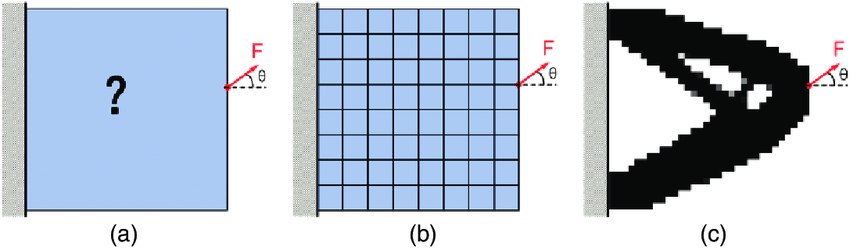
\includegraphics[width=1.0\linewidth]{./figures/intro-simp}
    \caption{2D SIMP拓扑优化方法示意图~\cite{luo_simp2021}}
    \label{fig:simp}
\end{figure}
\subsection{匀质化方法}
均匀化理论是一种确定等效均匀化材料属性的方法。1988年,Bendsoe和Kikuchi提出了首个连续体结构拓扑优化的均匀化方法\cite{BENDSOE1988}。该方法将宏观结构划分为单元胞,以单元胞结构属性(如材料密度、弹性模量、几何尺寸等)作为设计变量,将拓扑优化问题转化为单元胞微结构尺寸优化问题。随后,他们又提出了二维和三维结构的均匀化方法\cite{GUEDES1990}。
Michel等人利用均匀化方法研究了复合材料周期微结构的计算方法\cite{MICHEL1999}。吴长春等人采用均匀化方法优化了复合材料的极值弹性特性和最大刚度,实现了微结构的拓扑优化设计\cite{Yuan2003}。谢天海等人利用均匀化方法对柔顺结构进行了拓扑优化研究\cite{Xie2003}。王晓明等采用均匀化理论和伴随变量法分析了连续体结构拓扑优化的灵敏度,表现出良好的数值计算性能\cite{Wang1999}。
需要注意的是,由于均匀化方法存在构造微结构和设计变量过多等问题,其主要应用于材料微观设计领域。
\subsection{SIMP方法}
变密度法是在均匀化方法基础上发展而来。该方法将设计域离散为有限单元网格,以每个单元或节点的相对密度作为设计变量,利用密度惩罚方法使相对密度在1和0之间连续变化。
SIMP方法(实体各向同性材料惩罚模型)是一种基于变密度法的拓扑优化方法,如图~\ref{fig:simp}所示,展示了SIMP拓扑优化方法的一个2D示例。SIMP方法最早由Rozvany等人提出\cite{Rozvany1992}。他们验证了SIMP方法的最终优化结构与采用均匀化方法得到的结果一致。Sigmund和Bendsoe探索了多种变密度法材料插值模型\cite{Bendsoe2003,Bendsoe1999},指出SIMP方法中产生的中间密度值具有物理意义,并验证了指数形式的材料插值模型具有广泛适应性。Rozvany等人详细介绍了SIMP方法的起源、理论背景及主要优缺点\cite{Rozvany2001}。
Yuan等人在变密度法中成功引入了杂交单元,实验结果表明可获得更优的拓扑优化结果,并克服了棋盘格现象\cite{Yuan2001}。李翔等人提出过滤函数方法来解决SIMP方法中灰度单元过多的问题。Martinez等人研究了SIMP方法的收敛性,给出了更弱的假设条件\cite{Martinez2005}。
变密度法具有较强的普适性,适用于各类拓扑优化问题,因此在连续体结构拓扑优化中应用广泛。


\subsection{水平集方法}
水平集方法最早主要应用于图像处理和流体力学中的运动边界跟踪,由Sethian和Osher等人提出~\cite{OSHER1988,OSHER2001}。如图~\ref{level-set}所示,其主要思想是将移动边界作为零水平集嵌入高维水平集标量函数中,这样就可以利用闭曲面演化的方法得到水平集函数的演化方程,而嵌入的闭曲面总是其零水平集,最终只需确定零水平集即可确定移动界面的演化结果。
水平集方法具有几何直观性强、能够处理拓扑变化等优点,因此在结构优化领域也得到广泛应用。2000年,Sethian等人将水平集方法成功应用于结构优化~\cite{SETHIAN2000}。Wang等人利用方向导数进行灵敏度分析,将水平集方法应用于均匀材料、多材料、柔性机构的拓扑优化设计~\cite{Wang2003,Wang2004}。庄春刚等人比较了水平集方法与SIMP方法,指出水平集方法得到的优化结果具有光滑的几何边界,数值算法更稳定~\cite{zhuang2007}。
此外,水平集方法还被应用于结构形状优化、多目标优化、动态优化等领域。
\begin{figure}[htpb]
\centering
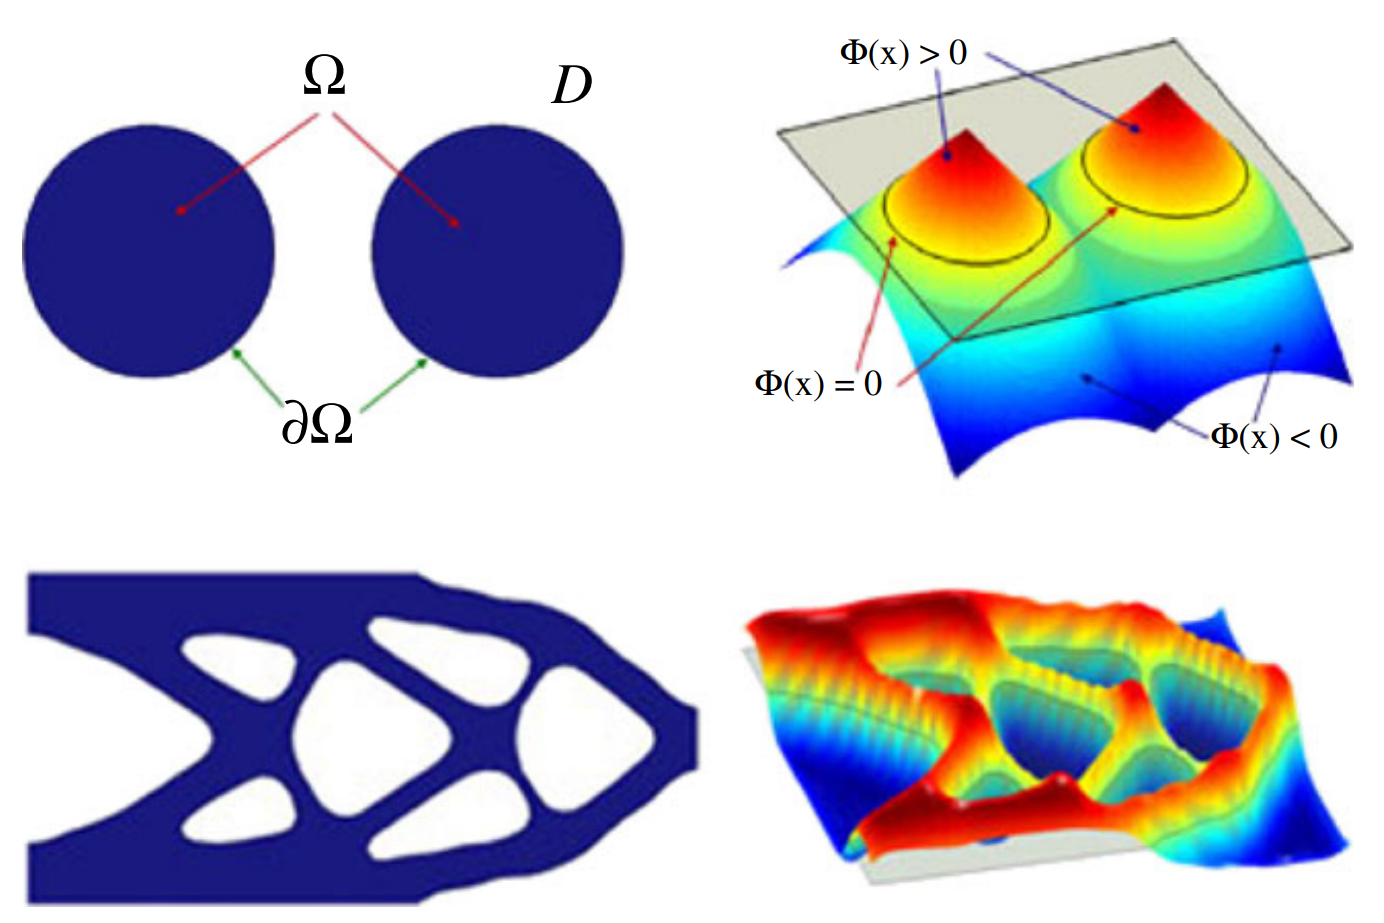
\includegraphics[width=0.9\linewidth]{./figures/intro-level}
\caption{水平集方法~\cite{deaton2014survey}}
\label{level-set}
\end{figure}

\subsection{MMC/MMV方法}
从几何表示的角度来看,以上方法都是在基于像素或节点的求解框架内开发的。这些方法虽然取得了显著的成果,但仍存在一些具有挑战性的问题需要进一步解决:
首先,基于像素的拓扑表示与现代计算机辅助设计(CAD)建模系统并不完全一致,因此无法直接在CAD平台上进行优化。其次,由于基于像素的拓扑优化方法没有明确嵌入几何信息,很难对结构特征尺寸进行精确控制,而在制造方面,这一点通常很重要。最后,采用单元材料分布来表示结构拓扑,基于像素的拓扑优化方法所涉及的计算工作量相对较大,特别是在三维问题中,所需的计算量大得难以想象。水平集方法是基于节点的拓扑优化方法的代表。在水平集方法中,也需要将设计域离散为有限元来计算结构响应,但通常以节点处的水平集函数值作为拓扑设计变量。虽然几何信息(如外法向量和曲率边界等)可以从水平集函数计算,但水平集方法在CAD建模系统中采用的隐式几何表示方式与显式几何表示方式有很大不同,因此基本上具有与变密度法相同的缺点,也无法摆脱维度魔咒。
\begin{figure}[htpb]
\centering
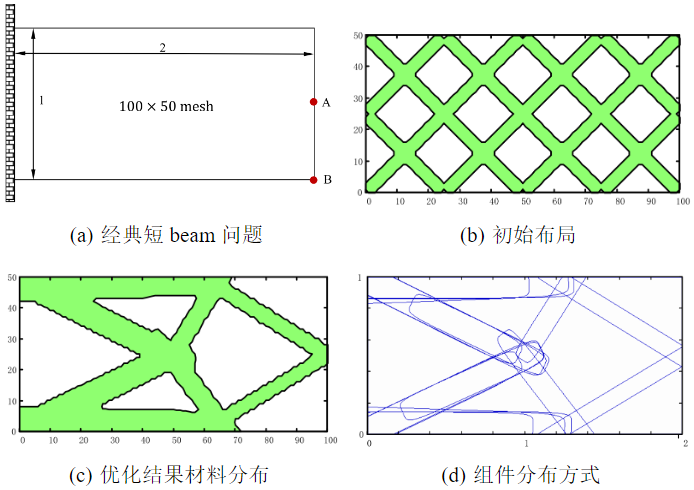
\includegraphics[width=1.0\linewidth]{./figures/intro-mmc}
\caption{可移动变形组件方法~\cite{Zhang2014}(MMC)}
\label{MMC}
\end{figure}
\begin{figure}[htpb]
\centering
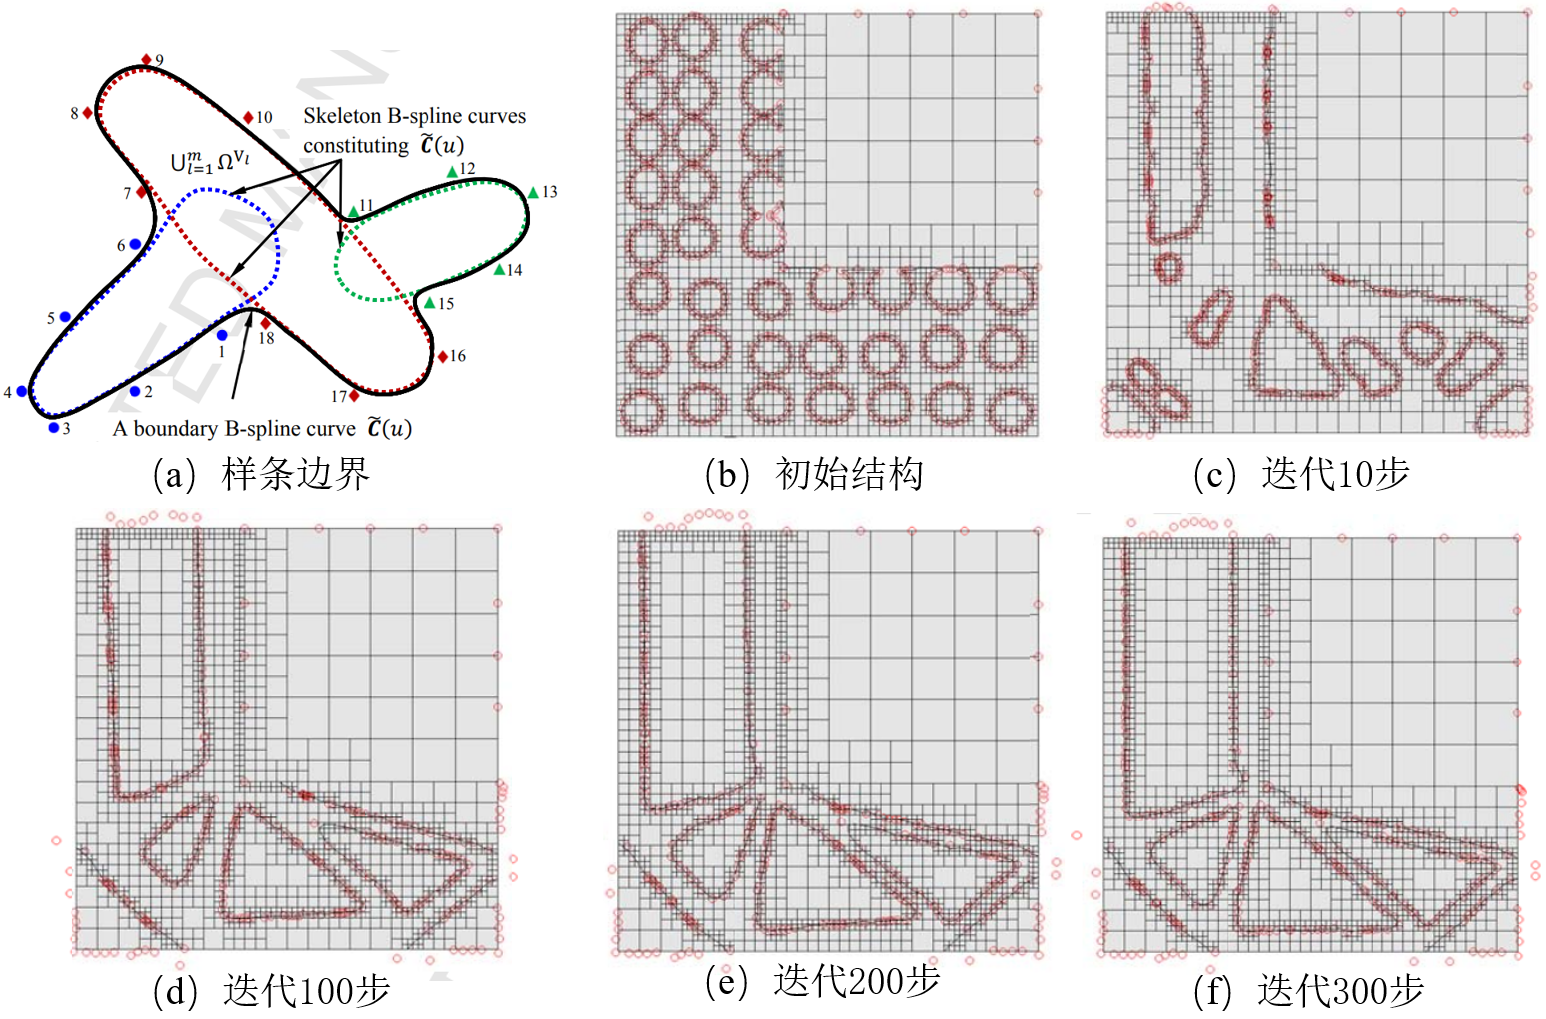
\includegraphics[width=1.0\linewidth]{./figures/intro-mmv}
\caption{可移动变形孔洞方法~\cite{zhang2018moving}(MMV)}
\label{MMV}
\end{figure}
为了建立结构拓扑优化和CAD建模系统之间的直接联系,Guo等人提出了一种更几何化、更灵活的显式化方法——可移动变形组件方法(MMC)~\cite{Zhang2014}。该方法的显著特点是使用一组可变组件作为拓扑优化的构建块,通过优化这些组件的形状、长度、厚度、方向和布局(连通性)来找到最优的结构拓扑。如图~\ref{MMC}所示,对于经典的短梁问题,在A点受竖直向下的力,先在设计域中给定初始的组件分布,然后通过优化得到最终的拓扑优化结构,图~\ref{MMC}(d)显示的就是最终组件的分布方式,由此决定了优化结构的布局。随后,Zhang等人又提出了对偶的可移动变形孔洞方法,如图~\ref{MMV}所示。该方法用样条来确定孔洞的边界,然后通过优化多个样条参数来获取设计域上挖洞区域的确定,从而达到结构优化的目的。

MMC/MMV这种显式方法的一大优点是可以将CAD建模系统的尺寸、形状和拓扑优化无缝地集成在一起,这在工程应用中具有很大潜力。此外,与SIMP、水平集方法相比,它拥有较少的优化变量,在计算上表现出较高的效率和鲁棒性。


\section{结构表示}
结合以上拓扑优化算法的现状分析可以看出,结构的表示方式一定程度上决定了拓扑优化方法的特点和性能,比如SIMP方法中的结构是基于单元密度表示的离散方法,而水平集方法中的结构是基于水平集函数表示的 连续方法。表示方法不同,拓扑优化的优化参数不同。在计算机图形学中,三维几何体通常用网格、样条、点云等方法来表达~\cite{agoston2005computer},这些方法用三角网格、三维点或者样条曲线曲面等基本元来描述几何体的边界,被称为显式表示。与之相区别的是隐式表示,其通过定义一个三维空间中的隐式场函数来表示几何体。
\begin{figure}[htbp]
    \centering
    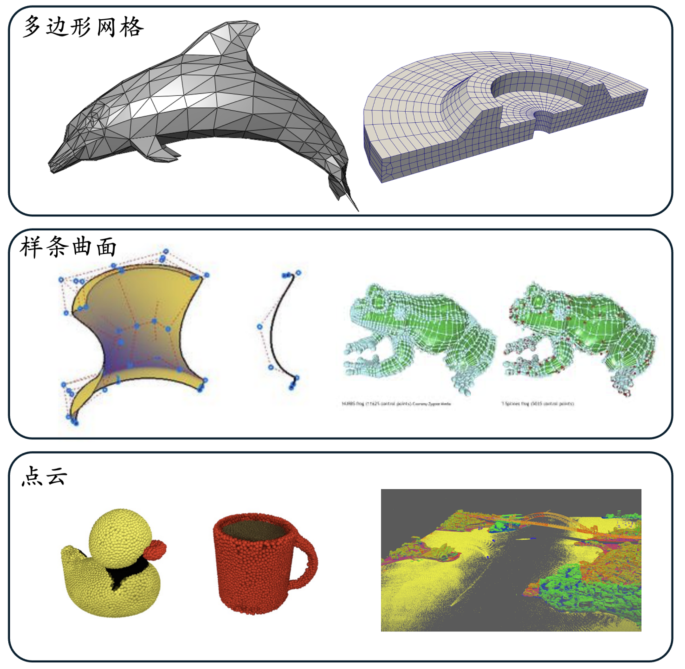
\includegraphics[width=0.48\linewidth]{./figures/intro-explicit-rep}\hfill
    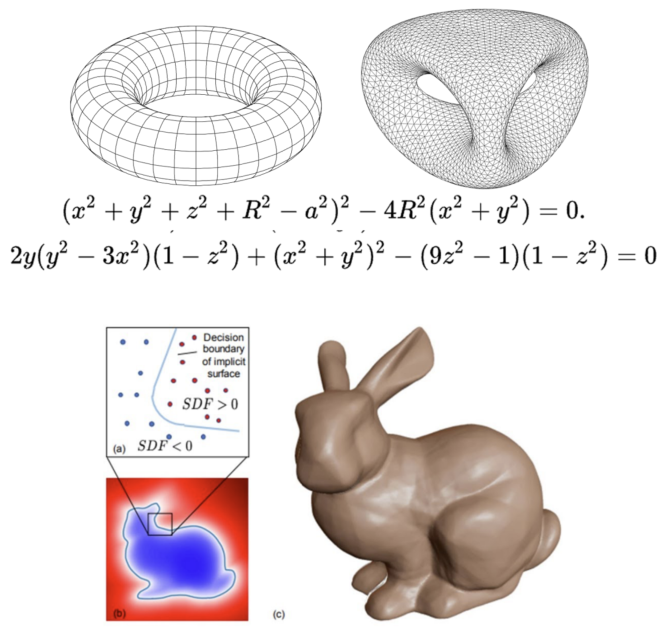
\includegraphics[width=0.48\linewidth]{./figures/intro-implicit-rep}
    \\
    \makebox[0.48\linewidth]{(a)显式表示}
    \hfill
    \makebox[0.48\linewidth]{(b)隐式表示}
    \caption{三维结构的不同表示方法}
    \label{fig:structure-rep}
\end{figure}
\subsection{显式表示}
多边形网格表示是描述三维几何方法中最常用的一种方式,尤其是三角网格表示,如图~\ref{fig:structure-rep} 所示。网格表示的基本元素包括顶点、边和面,这种表示的优点是比较直观,可以表示任意复杂的几何形状,能够通过局部增加顶点和面来精确地描述物体的形状和细节。计算机图形学中也有很多成熟的网格处理算法~\cite{botsch2010polygon},用于几何的表示、变形和布尔等操作。
但是复杂的几何形状需要大量的顶点、边和面等元素信息,导致数据量增大,而且网格表示难以处理具有复杂几何和拓扑特征的几何操作。

在计算机辅助设计(CAD)中,样条表示是一种常用的方法,其通过一组控制点定义的光滑曲线或曲面,能够精确地表示自由形状,常用的有B\'ezier曲线,B-样条和NURBS样条等~\cite{eck1996automatic,熊运阳2014cad},随后发展起来的T-样条克服了传统NURBS样条的局限性~\cite{sederberg2003t,李新2008t},进一步提高了建模的灵活性和效率。样条表示在几何建模中具有显著的优点,包括生成高质量的曲线和曲面、提供灵活的局部控制能力以及能够精确表示形状。然而,其计算和实现的复杂性较高,特别是在处理非光滑特征和局部修改时可能引发全局变化。此外,样条在不同CAD系统之间的兼容性也往往会发生问题。

点云是另一种被广泛应用的三维几何表示方法,其由存在于几何表面的点集合构成~\cite{杨必胜,ran2022surface},除了存储点坐标信息之外,有时还包含其他属性如颜色、法向量等。点云通常通过三维扫描仪、激光雷达等设备获取。点云表示作为一种几何表示方法,具有数据获取便捷、精确度高、灵活性强以及能够直接表示三维空间等优点,但同时也存在数据量大、缺乏拓扑信息、噪声敏感和处理复杂等缺点。这种表示方式在三维重建、自动驾驶~\cite{cui2021deep}、虚拟现实和机器人导航等领域具有广泛应用,尽管面临一定的技术挑战。

\subsection{隐式表示}
几何的隐式表示是一种通过数学函数来描述几何形状的方法。与显式表示不同,隐式表示不直接存储几何体的顶点和边等确定边界的信息,而是通过一个函数来定义几何体的形状。常见的隐式表示包括隐式曲面,距离场(SDF)~\cite{park2019deepsdf,yang2021geometry}和占用率场(Occupancy Field)~\cite{mescheder2019occupancy}等,如图~\ref{fig:structure-rep} (b) 所示。隐式表示使用一个标量函数$f(\mathbf{r})=s$来定义几何体,其中$\mathbf{r}=(x,y,z)\in\mathbb{R}^3$是空间中的坐标。具体来说,对于占用率场,其定义为,
\begin{equation}
f(\mathbf{r})=
    \begin{cases}
        0, & \text{如果}\mathbf{r}\text{是在几何体外部},\\
        1, & \text{如果}\mathbf{r}\text{是在几何体内部}.
    \end{cases}
\end{equation}
而对于有向距离场,其定义为,
\begin{equation}
f(\mathbf{r})
    \begin{cases}
        >0, & \text{如果}\mathbf{r}\text{是在几何体外部},\\
        =0, & \text{如果}\mathbf{r}\text{是在几何体边界},\\
        <0, & \text{如果}\mathbf{r}\text{是在几何体内部},\\
    \end{cases}
\end{equation}
其值代表空间坐标$\mathbf{r}$到几何体表面的最短距离,并通过符号区分几何体的内部和外部。隐式表示通常只需要一个函数即可描述复杂的几何形状,比显式表示更为紧凑,而且几何体之间的布尔运算可通过简单的函数操作即可实现,但是隐式表示的几何体描述不如显式表示直观,理解和操作较为困难。

总的来说,几何的隐式表示是一种强大且灵活的几何描述方法,适用于描述具有复杂形状和拓扑的几何体,但其求解和存储的复杂性也对计算资源和算法提出了较高的要求。

\subsection{隐式神经表示}

\section{基于深度学习的拓扑优化方法}
\begin{figure}[htbp]
    \centering
    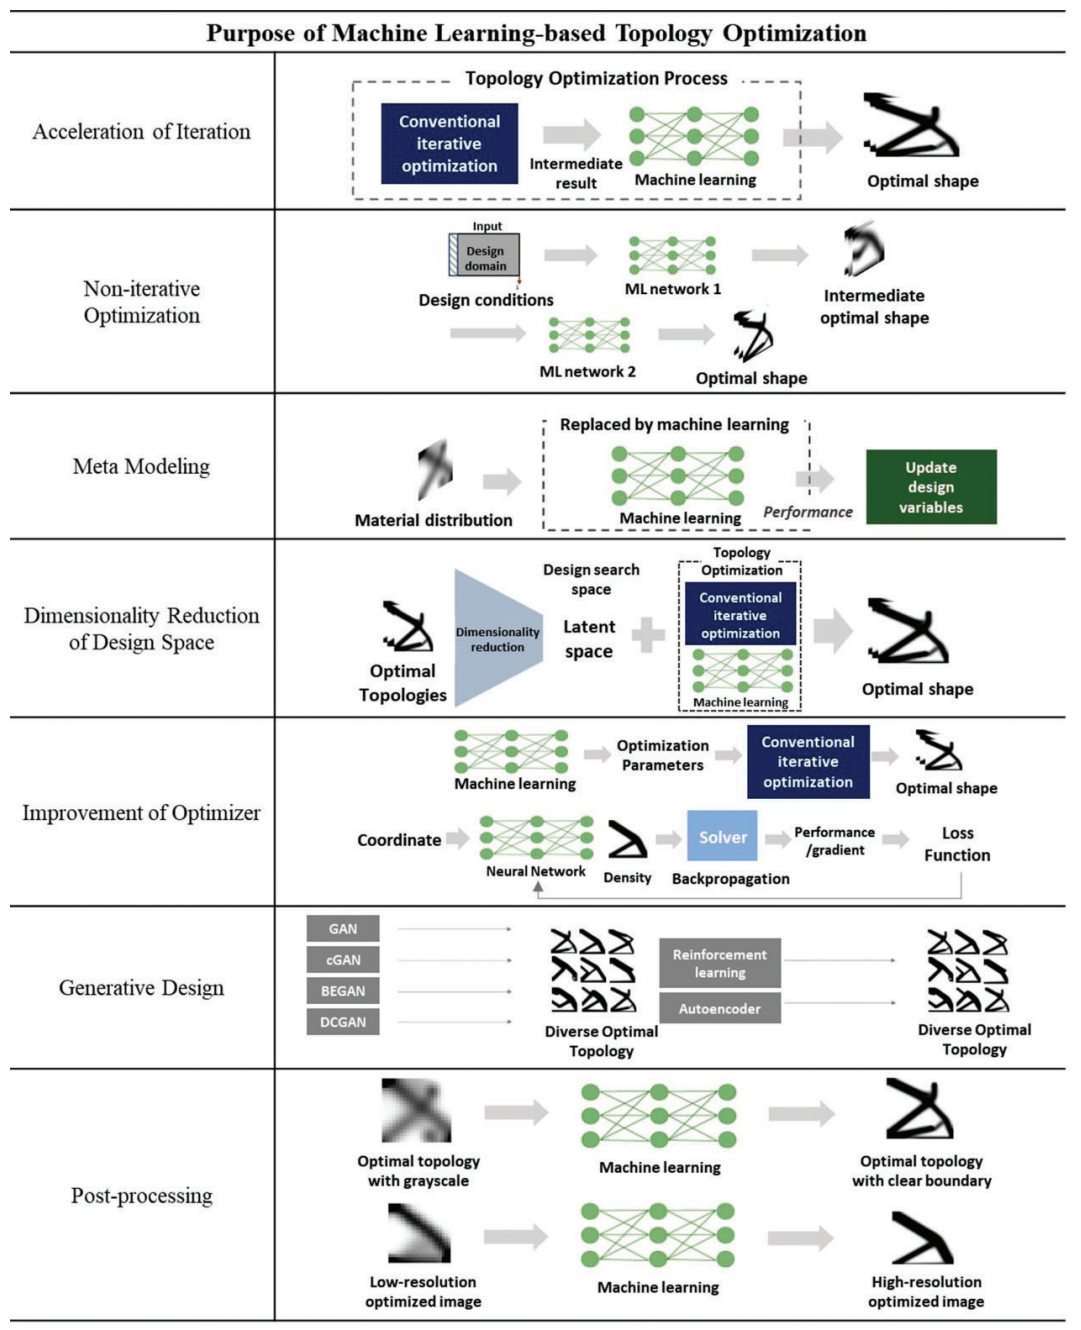
\includegraphics[width=1.0\linewidth]{figures/TOwDL.png}
    \caption{拓扑优化使用学习方法的常见途径~\cite{shin2023topology}}
    \label{fig:TOwDL}
\end{figure}
虽然拓扑优化被认为是一种有效的逆向设计方法,但它面临的一个关键挑战是有限元分析所需的高计算成本;每次迭代优化都必须计算敏感度信息以指导参数调整。对于精细结构的优化,网格分辨率的提高也会导致分析时间显著增长,特别是在解决实际三维问题时,这一挑战尤为突出。因此,众多研究致力于提高拓扑优化的效率,其中神经网络驱动的设计优化方法近年来受到了广泛关注,成为了一个有效的解决途径。如图~\ref{fig:TOwDL} 所示,学习方法目前被用于拓扑优化中用来加速或者改善解的最优性等。
基于神经网络的方法通过其非线性建模能力,将复杂的高维结构优化问题转化为神经网络的参数优化问题,利用梯度反向传播算法和数值优化技术实现结构的快速设计。神经网络加速的拓扑优化方法主要分为两类:

第一类采用端到端的方式,在既定目标和约束条件下直接预测最优化结构,以非迭代的策略实现效率的显著提升。大部分方法将基于密度表示的结构看作二维或三维张量,并利用卷积神经网络(CNN)提取特征,接着通过变分自动编码器(VAE)或者对抗生成模型(GAN)学习结构的特征分布,最后在条件设定下利用学习到的分布直接生成最优结构。最近,在文本图像生成领域取得巨大成功应用的扩散模型(DDPM)也被扩展到端到端拓扑优化算法研究中,大幅提升了准确性和优化效率。

第二类提高效率的方法是利用神经网络替代传统迭代优化过程中耗时的有限元计算和敏感度分析。物理信息神经网络(PINN)是最近备受关注的新兴技术,它通过将物理定律直接嵌入到网络训练中,可以有效地模拟复杂系统的行为,从而规避了传统有限元方法中网格剖分和迭代求解步骤。许多研究已经将 PINN技术与拓扑优化方法相结合,用以替代传统有限元计算,从而提升优化过程的效率。Lee等人通过训练两个独立的 CNN 网络来预测结构的柔度和体积分数,并采用最优性标准(OC)方法更新设计参数。受到图像处理中超分辨率技术的启发,另一种方法利用神经网络从粗精度下的优化结构预测高精度的最优结构,这种方法通过减少维度显著提升了拓扑优化的计算效率。

近期,研究人员已经开始探索利用神经网络技术来设计和优化多孔结构。Kim 等人开发的 ZeoGAN 模型训练了三个神经网络以预测组合数据,成功模拟出真实沸石材料的微孔结构。Kumer 等人采用两个多层感知机(MLP)逆向设计出非周期性的旋转对称细胞结构,并对多孔结构的参数和刚度进行了交叉验证。此外,一些研究利用 VAE 和 GAN 等生成模型实现从图片中重建出多孔结构。Zhang 等人提出了一种整合 VAE 和 GAN的混合模型,提高了从图片生成三维多孔结构的稳定性,并通过引入孔隙损失来提高重建的准确性。超材料是多孔结构的直接应用之一,最近也有许多工作利用神经网络进行超材料单元结构的逆向设计。Wang 等人采用数据驱动的方式,在超材料数据库上训练VAE 模型及用于属性预测的回归器,将复杂的微观结构映射到低维度的连续隐藏空间中,通过简单的空间插值和遍历就可以生成丰富的新型超材料单元孔洞结构。IHGAN结合了GAN生成模型和传统均质化技术,创造出多样化的单元结构,相对于传统密度单一型结构显著提高了超材料结构的性能。然而,现有的神经网络驱动多孔结构设计方法很难与仿真和优化模块整合,这一步骤对于得到满足理想属性的多孔结构并将其应用到实践中至关重要。

\section{本文研究思路及目标}
\chapter{基于隐式表示的薄壳结构雕刻设计}

\section{引言}
薄壳结构以其纤薄和弯曲的形状承载载荷,这种结构特别优雅和高效。它们在我们的生活环境中以各种尺寸广泛存在,在满足力学性能的同时提供了艺术美感的视觉体验~\cite{adriaenssens2014,melaragno2012}。近年来,基于壳体结构的曲面设计受到艺术家和研究人员的广泛关注~\cite{Pietroni2015, Chen2016, Liu2020}。其中,雕刻是设计壳体结构的一种流行方式~\cite{Yang2019,stadlbauer2020}。经过精巧的雕刻设计,壳体结构可以具有更高的艺术感,并在医疗和轻量化应用中得到广泛实践~\cite{Zhang2017,Rao2019}。

现代计算机图形学技术的发展已经引领了壳体结构雕刻设计方法的日益多样化,例如基于纹理合成的方法~\cite{Dumas2015},基于镶嵌的方法~\cite{Pietroni2015}和基于重复模板的方法~\cite{schumacher2016}。作为一种材料减少过程,雕刻设计的核心问题是在设计过程中维持壳体结构的力学性能和功能。现有的大多数方法都侧重于显式表示,如多边形网格等,这不利于结构分析和参数优化。
由于雕刻壳体结构的拓扑和几何结构高度复杂,采用传统有限元方法(FEM)~\cite{bucalem1997,cirak2002} 进行力学响应分析非常耗时。此外,在现有的设计技术中,设计、分析和优化通常是分离的,在不同阶段经常需要重复重新划分网格~\cite{panetta2019}。由于缺乏统一的表示方法和有效的优化技术,在壳体结构上进行雕刻设计并非易事。

本文研究提出了一种隐式参数化方法来设计轻量级薄壳结构,并通过参数优化保证结构的物理可靠性,如图~\ref{fig:thin-shell-1} 所示。具体地,通过在输入薄壳结构上分布重复模板图案并对其进行雕刻来完成设计,用隐式表示的薄壳结构的模板图案可以直接用函数进行设计、分析和优化,本文通过优化模板图案的尺寸和方向等属性,在雕刻设计的同时最大化壳体结构的刚度。与基于传统有限元的网格方法相比,本文方法由于避免了显式模型的生成和分析过程中的重新网格剖分,在保证足够精度的前提下大大提高了计算效率。此外,本文还通过对图案模板的不同函数操作,实现了对偶雕刻设计,进一步增强了薄壳结构设计的丰富性。本文通过在多种薄壳结构模型上的测试,并实施了仿真和对比试验来证明该方法的有效性和高效性。

\begin{figure}[!b]
    \centering
    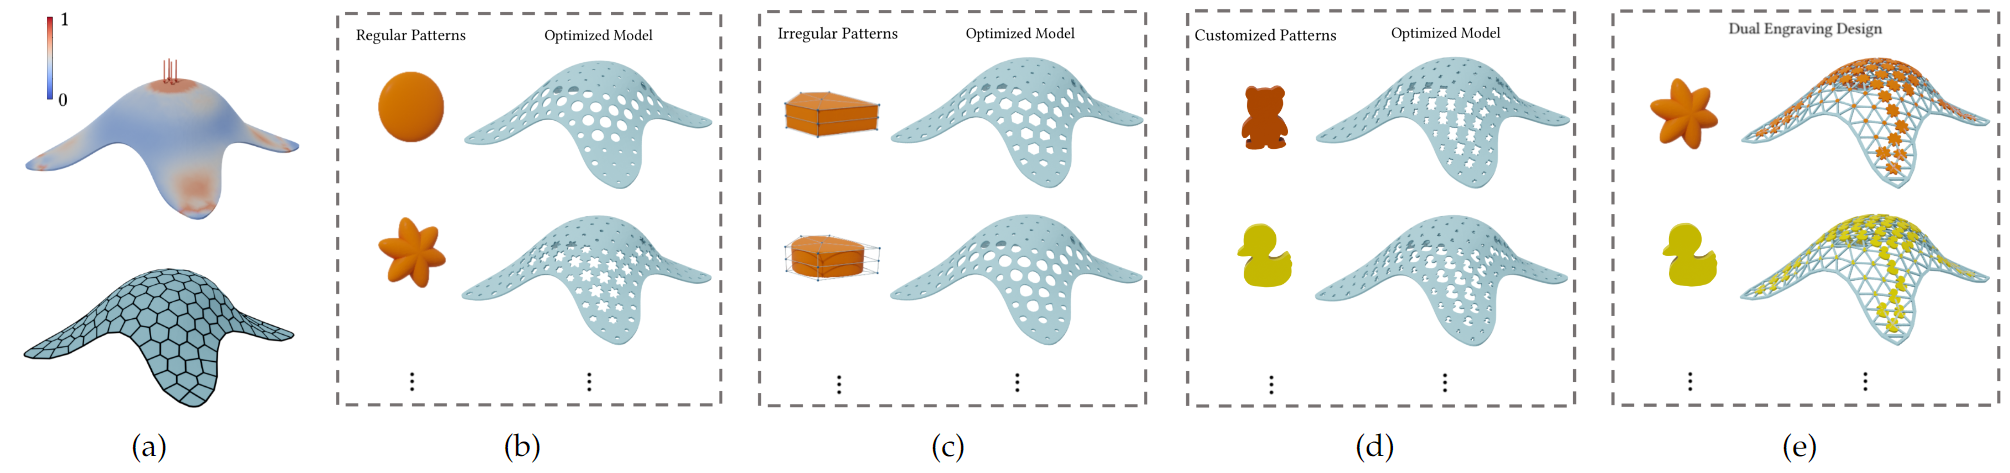
\includegraphics[width=1.0\linewidth]{./figures/thin-shell-1}
    \caption{基于隐式表示的                              薄壳(对偶)雕刻设计优化方法}
    \label{fig:thin-shell-1}
\end{figure}

\section{研究方法}

本方法基于结构的隐式表示设计了一种用于薄壳结构雕刻设计的参数化方法,算法流程如图~\ref{fig:thin-shell-pipeline} 所示。首先,使用函数表示构建三种类型的图案模板,包括规则图案、不规则图案和用户指定的个性化图案。这些图案模板具有可调整的属性, 例如位置、方向和大小, 可以通过参数控制(第~\ref{subsec:parametric-design}节)。然后,将这些模板图案用于壳体结构的雕刻。由于使用有向距离场(SDF)表示输入壳体,因此可以在图案模板和壳体模型之间执行函数布尔运算。最后,为了确保雕刻壳体结构的完整性,引入了结构力学问题的优化模型。以最小应变能为目标,给定体积为约束,该框架可以根据结构响应分析优化图案的属性变量。优化后的(对偶)雕刻壳体结构可以简单地用函数的零等值面表示(第~\ref{}节)。在各种壳体模型上成功实现了该算法,并进行了多组实验,验证了该框架的有效性和鲁棒性(第~\ref{}节)。


\begin{figure}[htbp]
    \centering
    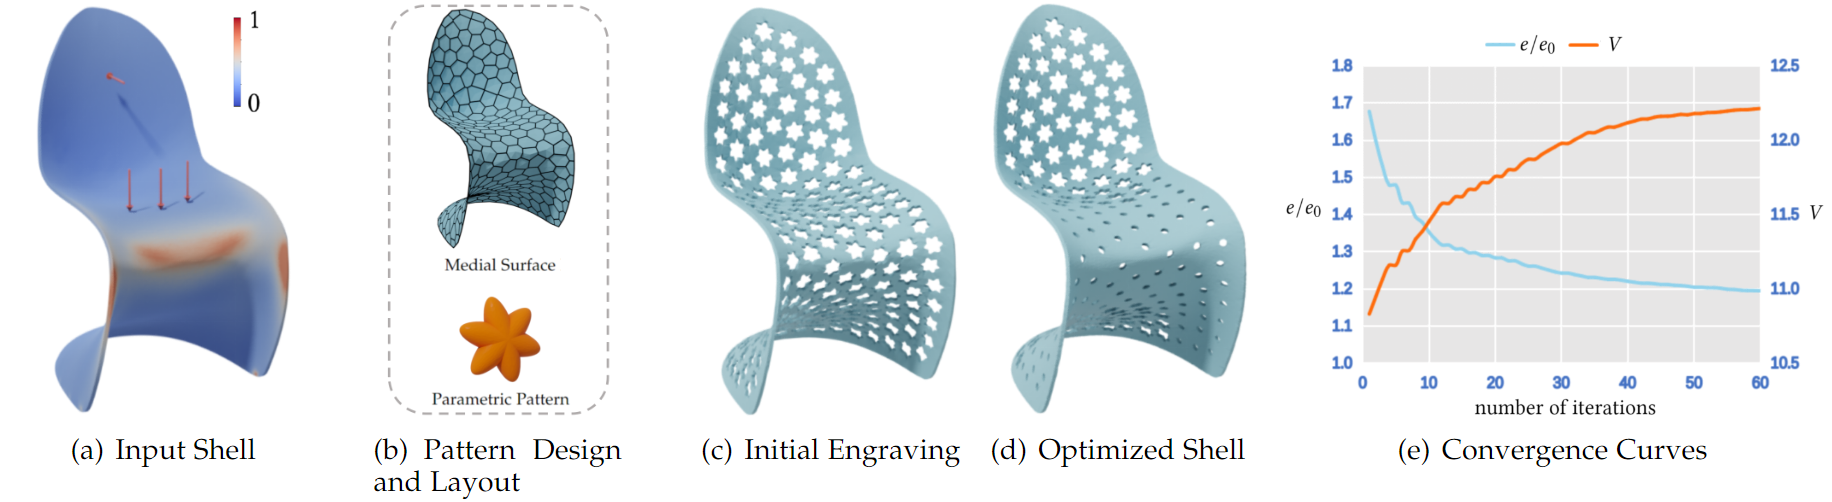
\includegraphics[width=1.0\linewidth]{./figures/thin-shell-pipeline}
    \caption{薄壳雕刻设计方法流程图}
    \label{fig:thin-shell-pipeline}
\end{figure}


\subsection{参数化设计}
\label{subsec:parametric-design}
本文算法采用隐式函数来表示输入模型和图案模板,从而将复杂的结构优化转化为可控参数设计问题,如此便可以高效、鲁棒和可扩展的方式进行结构的设计和优化。

\subsubsection{图案模板设计}
本文提出了三种用于薄壳结构雕刻设计的图案模板类型,包括规则图案、非规则图案和个性化图案,所有这些图案都可以用隐式函数表示。

\paragraph{规则图案。}首先考虑旋转对称的规则图案,并使用超椭球方程构造它们,
\begin{equation}
    \label{eq-ellipsoid}
    E(\mathbf{r})=\left(\frac{\hat{x}}{L_1}\right)^p+\left(\frac{\hat{y}}{L_2}\right)^p+\left(\frac{\hat{z}}{L_3}\right)^p-1,
\end{equation}
其中 $\mathbf{r}=(x, y, z)^\top\in\Omega$ 为三维空间 $\mathbb{R}^3$ 中的设计域,  $\mathbf{c}_0=(x_0,y_0,z_0)^\top$ 是超椭球的中心坐标。
定义 $\hat{\mathbf{r}}=(\hat{x}, \hat{y}, \hat{z})^\top=\mathbf{R}(\mathbf{r}-\mathbf{c}_0)$, 其中 $\mathbf{R}=\{R_{ij}\}_{3\times 3}$ 为旋转矩阵用于调整超椭球的方向。 $L_1$,$L_2$,和 $L_3$ 是超椭球的三个轴长,$p$ 是形状因子,是一个大于零的偶数。当 $p$ 增大时,超椭球逼近一个长方体。

通过控制少量参数,多个超椭球可以构成丰富复杂的图案结构。可以在局部坐标系中围绕其中心点旋转一个超椭球,以获得新的图案, 如图~\ref{fig-ellip} 所示。Specifically, assuming that a pattern is composed of $n$ super-ellipsoids $\{E_i\}_{i=1}^n$, the rotation angle of the $k$-$th$ super-ellipsoid should be $\frac{k\pi}{n}$, $k=1,2,\cdots,n$. 
We compute the orientation of super-ellipsoid $E_k$ by the rotation matrix $\Lambda(\frac{k\pi}{n})\mathbf{R}$, where $\Lambda(\theta)$ is the $z$-axis rotation matrix 
% !TeX root = ../thuthesis-example.tex

\chapter{基于隐式表示的自支撑空心化轻量结构设计}

\section{引言}
空心化在计算制造中广泛应用,目的是在不改变外表面的情况下减少材料消耗和打印时间~\cite{plocher2019review}。3D打印方法如熔融沉积成型(FDM)通常需要额外支撑结构,以避免空心腔内大量悬空部分崩塌。这些额外支撑材料虽旨在支撑,但对结构强度增强有限,且在打印后从完全封闭内部空间去除存在挑战。因此,优化内部结构以增强强度,同时保持自支撑能力至关重要。
设计自支撑结构的方法包括后处理、带约束的反向设计和建模自支撑空腔。但后处理方法通常产生无法控制的填充比和脆弱构件。反向设计需考虑多约束,包括自支撑约束~\cite{zheng2023topology},导致计算复杂度高,难以找到最优解。近年来,通过设计自支撑空腔进行空心化的简单高效策略受到关注~\cite{lee2018support, wu2016self, wang2018support, xu2021support,liu2023self}。
现有方法基于空腔的显式表示~\cite{lee2018support, wu2016self},难以控制和广泛应用。这些方法仅考虑自支撑特性,未优化结构强度~\cite{lee2018support,xu2021support}或使用启发式优化~\cite{wang2018support},导致性能有限且不可靠。高效设计和优化自支撑空腔用于空心化仍是一大挑战。
与显式方法相比,函数表示的结构连续,可通过参数轻易控制~\cite{carr2001reconstruction, hu2020efficient}。直接对函数进行解析计算可避免优化过程中频繁重网格,大幅提高自支撑空心化的效率和效果。

本章节提出一种基于3D椭球体的自支撑空腔,用于空心化给定模型,可用函数表示并通过参数控制。由于椭球体的平滑性,该自支撑空腔能有效减少应力集中~\cite{2008Peterson}。所提出的算法利用函数表示,可直接对函数进行积分和梯度计算,避免耗时的重网格划分,仅需一次构建基本的均匀有限元,作为优化过程中的积分域。
具体而言,使用径向基函数和椭球体函数分别描述模型和空腔,通过操作函数可实现空心化过程,调整椭球体函数参数,可轻易改变空腔的位置、尺寸和自支撑特性。
如图~\ref{fig:1}所示,展示了该流程。初始时,根据给定载荷和边界条件下输入实体模型的应力场布置空腔。实验表明,良好的初始化有助于快速收敛。然后进行高效的优化过程,优化空腔的形状、位置和拓扑。最终得到具有优化自支撑空腔的空心化模型,具有最高刚度。并且,所有优化结构均可使用常见的FDM 3D打印技术完美制造。此外,一旦建立了封闭空腔之间的连接通道~\cite{yang2023differentiable},该框架可扩展到其他增材制造技术,如SLS和SLA。重要的是,该框架内所有的设计和优化过程均为全自动化。

\begin{figure*}[!t]
  \centering
  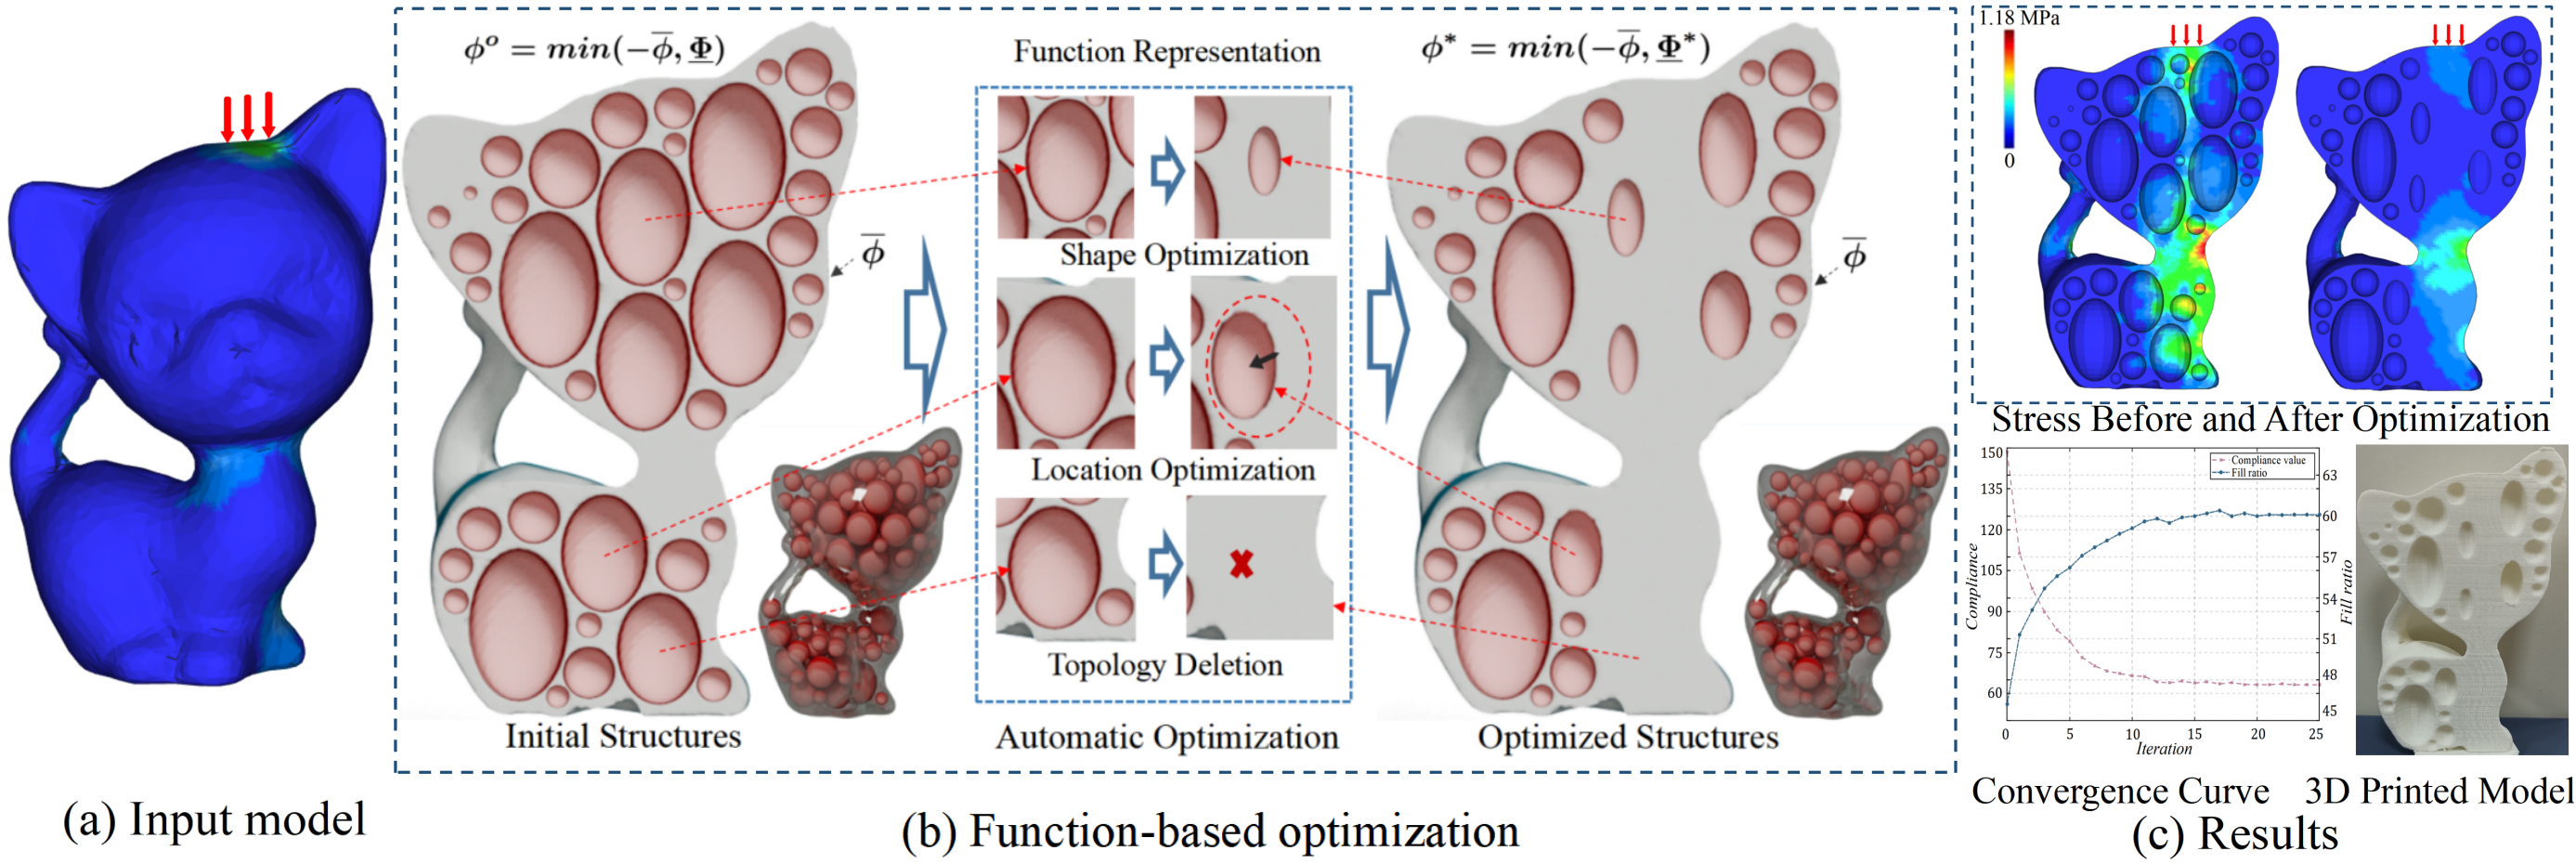
\includegraphics[width=0.95 \textwidth]{./figures/self-support/fig2.png}
  \caption{自支撑空心化算法流程图}
  \label{fig:1}
\end{figure*}

\section{研究方法}
以FDM 3D打印为例,在3D打印中有两个重要参数决定了打印模型的内部自支撑特性,分别是最大悬挑长度 $\delta_{0}$ 和最大悬挑角度 $\theta_{0}$,如图~\ref{fig:2}所示。这些与材料相关的参数 $\theta_{0}$ 和 $\delta_{0}$ 可通过实验测量得到。对于PLA材料,默认参数设置为 $\delta_{0}$ = 10mm 和 $\theta_0$ = $60^{\circ}$。

\subsection{自支撑空心结构设计}
本章算法在设计自支撑空心结构上,采用椭球体作为自支撑空腔结构,主要有两个原因:一是椭球体具有少量参数的显式函数表达式;二是可通过调整参数轻易实现自支撑。实际上,椭球体尺寸大小会影响其自支撑特性,如图~\ref{fig:2}所示。这意味着尺寸较小时,球体可无需支撑即可打印(图~\ref{fig:2} (b))。为更好描述自支撑椭球体问题,需引入一些定量参数:椭球体$E$在$X$、$Y$和$Z$轴上的三个主要半径分别为$a$、$b$和$c$;椭球体的打印方向默认与$z$轴对齐。为避免内部椭球体过小无法打印,设置$\min\{a, b\}> 5\sigma$,其中$\sigma$为每层制造厚度(默认$\sigma$=0.2 mm)。椭球体的下半球为自支撑,仅需考虑上半球。如图~\ref{fig:2} (a)所示,当悬挑角$\theta < \theta_{0}$时,相应部分为自支撑(低于红色水平线$p_1p_2$的部分)。对于悬挑角$\theta > \theta_{0}$的部分,若$p_1$和$p_2$间水平距离小于$\delta_{0}/2$,上方部分仍可自支撑。因此,可将椭球体自支撑的条件表述如下~\cite{lee2018support}:
\begin{equation}
  \begin{cases}
          a\leq c , \qquad &\text{if} \,\,  5\sigma \leq a \leq \delta_{0} / (2\ \cos\theta_{0}),                                       \\
          b\leq c , \qquad &\text{if} \,\,  5\sigma \leq b \leq \delta_{0} / (2\ \cos\theta_{0}),                                       \\
          c\geq a(4a^2-\delta^2_{0})^{\frac{1}{2}} \left. \middle/ \delta_{0}\ \tan\theta_{0} \right. \ \quad &\text{if} \, \, \, a > \delta_{0} / (2\ cos\theta_{0}),   \\
          c\geq b(4b^2-\delta^2_{0})^{\frac{1}{2}} \left. \middle/ \delta_{0}\ \tan\theta_{0} \right. \ \quad &\text{if} \, \, \, b > \delta_{0} / (2\ cos\theta_{0}). 
          \label{eq:1}
  \end{cases}
\end{equation}
\begin{figure}[htbp]
  \centering
  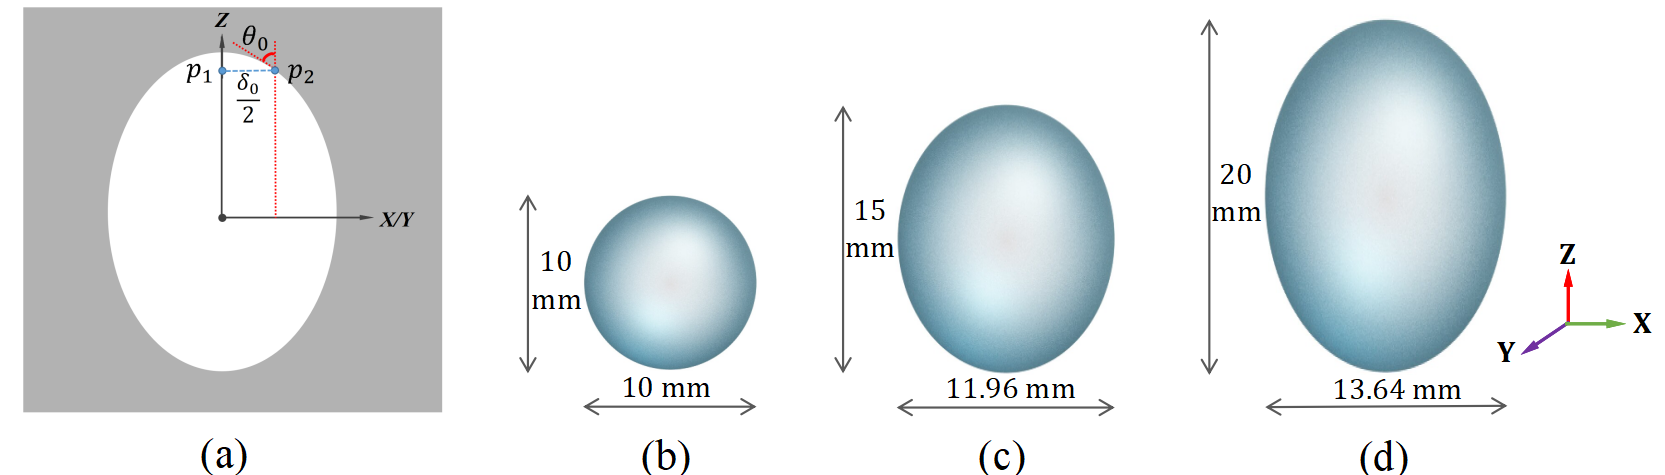
\includegraphics[trim={0 40 0 0},clip,width=0.65\textwidth]{./figures/self-support/fig3.png}\\
  \caption{自支撑椭球体示意图}
  \label{fig:2}
\end{figure}
对于固定主半径$c$的椭球体,可根据公式~(\ref{eq:1})调整另外两个半径$a$和$b$以获得自支撑的椭球体。图~\ref{fig:2} 还展示了具有不同尺寸的自支撑椭球体。在该方法中,确定可优化变量的范围对优化器很重要。

\subsection{自支撑空性化模型的函数表示}
相比离散边界表示,连续函数表示具有多方面优势,包括参数可控性、高精度、解析优化,以及易存储和传输。由于椭球体具有函数表示,可使用函数表示来描述具有椭球体空腔的模型。对于具有椭球体空腔的3D模型,可将其划分为模型的外表面和椭球体空腔的内部表面两部分,模型的外表面和内部表面均可使用函数进行隐式表示。
\begin{figure}[htbp]
  \begin {center}
  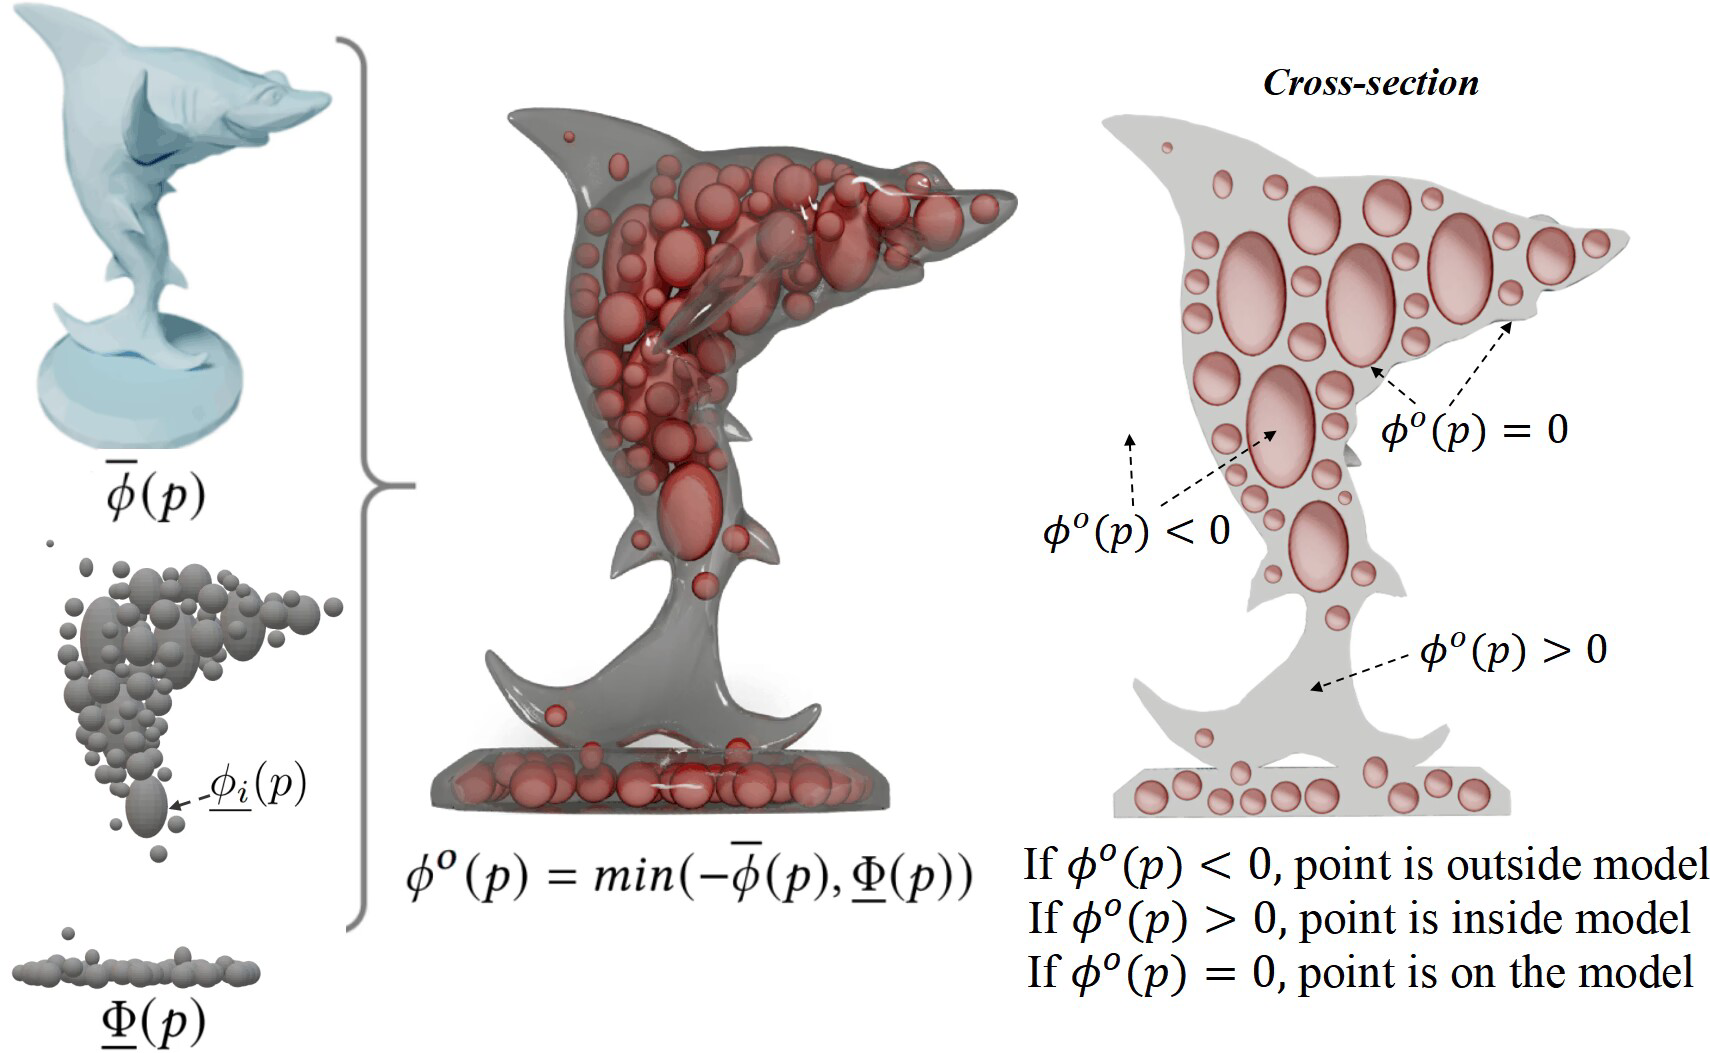
\includegraphics[width=0.65\textwidth]{./figures/self-support/fig4.png}
  \caption{椭球空心化3D模型的函数表示}
  \label{fig:3}
  \end {center}
\end{figure}

外表面可以用下面的径向基函数插值得到,
\begin{equation}
  \overline{\phi}(p)=\sum _{i=1}^{n_{t}}\alpha_{i}R_{i}(p)+Q(p),
  \label{eq:2}
\end{equation}
其中,$\overline{\phi}(p)$是模型的外表面函数,
$p=(x,y,z)$是设计空间中的一个点,
$R_{i}(p)=R(|p-p_{i}|)$是径向基核函数($R(x)=x^2log(|x|)$),
$\{p_{i}\}^{n_{t}}_{i=1}$是在模型表面上均匀采样的控制点集,
$n_{t}$是控制点的数量,
$Q(p)=\beta_{1}x+\beta_{2}y+\beta_{3}z+\beta_{4}$是一个单项式表达式,$\{\alpha_{i}\}$ 和 $\{\beta_{i}\} $ 是权重系数。
由于外表面无需改变,因此仅需对采样点和权重进行一次计算。该文采用RBF方法来逼近外表面,这是因为RBF具有强大的非线性拟合能力和高计算效率。当然,也可以考虑其他替代方案来实现相同的目标。

内表面通过椭球函数来表示,
\begin{equation}
  \begin{split}
      &\underline{\Phi}(p)=\min(\underline{\phi_{1}}(p), \underline{\phi_{2}}(p), \cdots, \underline{\phi_{n_e}}(p)),\qquad \quad
      \\
      &\underline{\phi_{i}}(p)=\frac{(x-x_{i})^2}{{a_i}^2}+\frac{(y-y_{i})^2}{{b_i}^2}+\frac{(z-z_{i})^2}{{c_i}^2}-1,
  \end{split}
  \label{eq:3}
\end{equation}
其中,$\underline{\Phi}(p)$表示椭球体空腔的整个内部表面,
$\underline{\phi_{i}}(p)$是第$i$个椭球体的表面,其三个主半径为($a_i$,$b_i$,$c_i$),中心点为$(x_{i},y_{i},z_{i})$,
${n_e}$是椭球体的数量,
$(x,y,z)$是椭球体的坐标,主半径和中心点用于控制椭球体,并根据目标需求进行优化。
然后,通过布尔运算可以获得具有椭球体空腔的3D模型的函数表示。具有椭球体空腔的3D模型的函数可表示为
\begin{equation}
  \phi^o(p)=\min(-\overline{\phi}(p), \underline{\Phi}(p) ). 
\end{equation}
函数表示可准确描述具有椭球体空腔的3D模型,并通过参数(如主半径和椭球体中心)控制其形状、位置和拓扑结构,图~\ref{fig:3}展示了具有椭球体空腔的模型表示。获得表示函数后,即可通过计算函数值轻松确定模型的内部和外部。若$\phi^o(p) < 0$,则点在模型外部;若$\phi^o(p) > 0$,则点在实体部分内部;若$\phi^o(p) = 0$,则点在模型表面上。连续可微函数有助于准确计算体积和进行高效敏感性分析,为自动优化提供可行条件。

\begin{figure}[t]
  \centering
  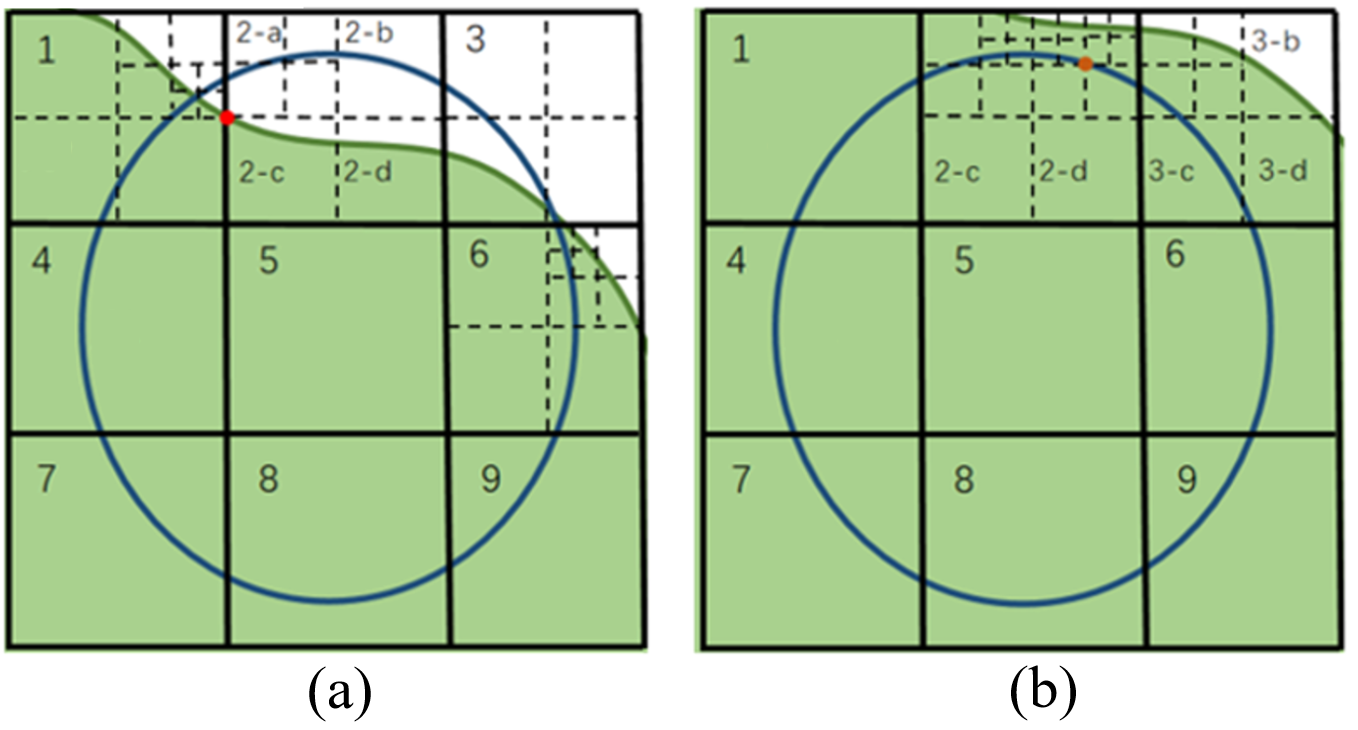
\includegraphics[width=0.6\textwidth]{./figures/self-support/fig6.png}
  \caption{2D视角下的自动定位示意图}
  \label{fig:5}
\end{figure}
\subsection{优化问题的形式及求解}
给定一个模型、外部载荷和体积约束,算法的目标是获得一个由椭球体组成的优化自支撑空腔的模型。所提出提出的问题形式和优化可以直接在函数上执行,无需耗时的重新网格化。结构柔度被用于制定优化目标,优化应变能以最大化结构刚度。在给定约束条件下,最小化具有自支撑空腔的模型顺应性可以表述如下:
\begin{equation}
  \begin{split}
      \min \quad  &I = \int_{\Omega_{D}} G(\phi^o(p))f \cdot u \, dV + \int_{\tau_{s}}F_{s} \cdot u\, dS ,     \\
      s.t.\quad  &\int_{\Omega_{M}} G(\phi^o(p)) \mathbb{E}:\, \varepsilon(u):\, \varepsilon(v)\, dV_{M}\\
      &= \int_{\Omega_{M}} G(\phi^o(p))f \cdot v \, dV  + \int_{\tau_{s}}F_{s} \cdot v\, dS,\,  \quad\forall v\in U_{ad},         \\
      & \int_{\Omega_{M}} G(\phi^o(p))\, dV< V_{c},                       \\
      & u = \overline{u} \quad on\quad \tau_{u},                       \\
      & d(\underline{\phi_{i}}(p), \underline{\phi_{j}}(p))>0,\forall \underline{\phi_{i}},\underline{\phi_{j}}\in\underline{\Phi},  \label{eq:7}
  \end{split}
\end{equation}
其中,$I$是结构顺应性,$\Omega_{D}$是设计域,$\Omega_{M}$是模型域,$G(*)$是正则化的Heaviside函数\cite{hu2020efficient},$f$是体积力,$F_{s}$是定义在Neumann边界$\tau_{s}$上的表面拉力,$v$是定义在$\Omega_{D}$上的相应测试函数,其中$U_{ad} = {v|v\in Sob_{1}(\Omega_{M}), v = 0 , on ,\tau_{u}}$,$u$是位移场,$Sob_{1}$是一阶Sobolev空间,$\varepsilon$是二阶线性应变张量,$\mathbb{E}$是由弹性模量和泊松比决定的四阶各向同性弹性恒等张量,$\overline{u}$是在Dirichlet边界$\tau_{u}$上的预设位移,$V_{c}$是体积约束,$d(\phi_{i}(p), \phi_{j}(p))$是第$i$个椭球体和第$j$个椭球体之间的距离。
\begin{figure}[t]
  \centering
  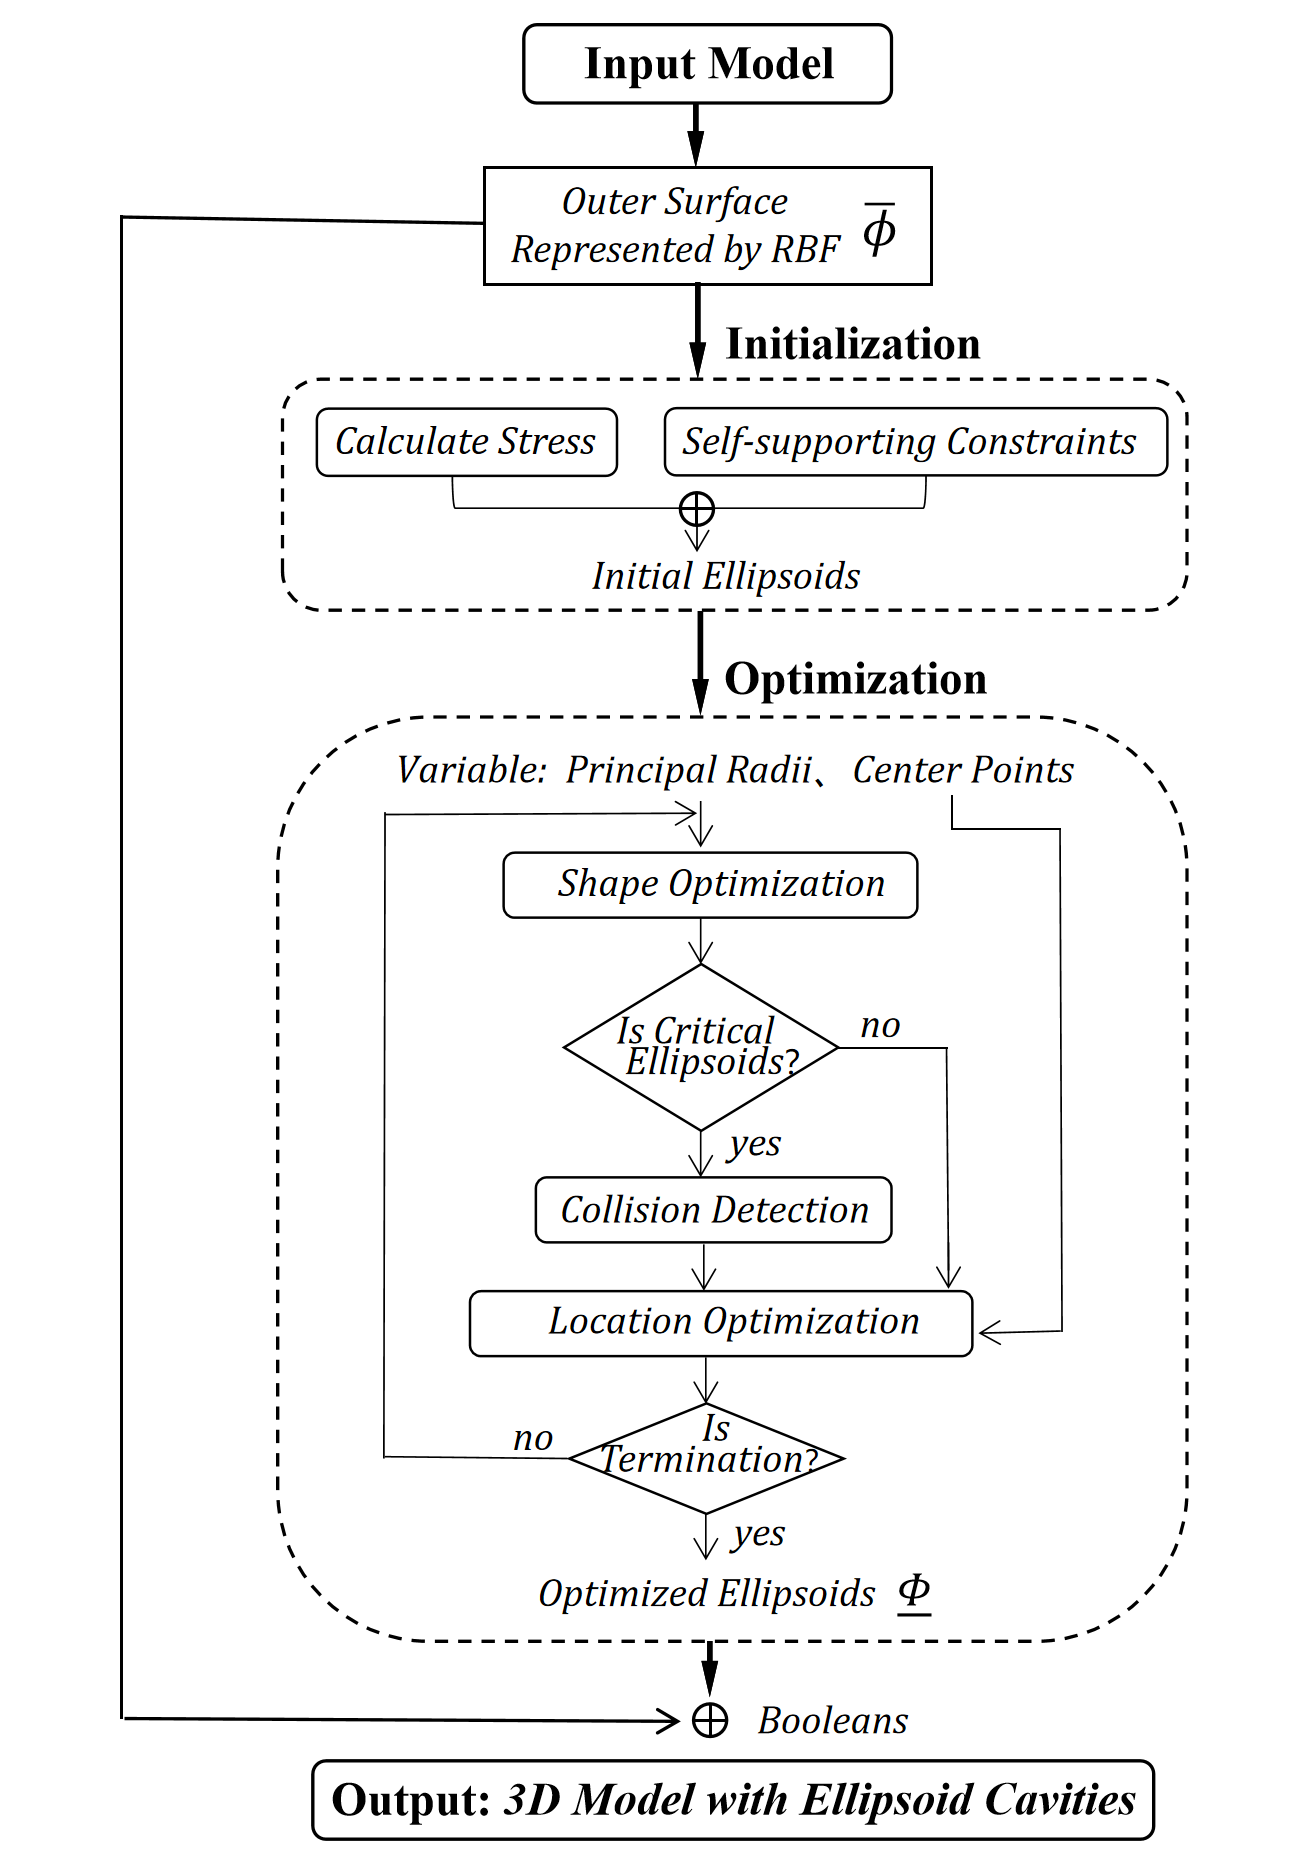
\includegraphics[height=4in]{./figures/self-support/fig17.png}
  \caption{算法流程}
  \label{fig:algo}
\end{figure}

\begin{figure*}[htbp]
  \centering
  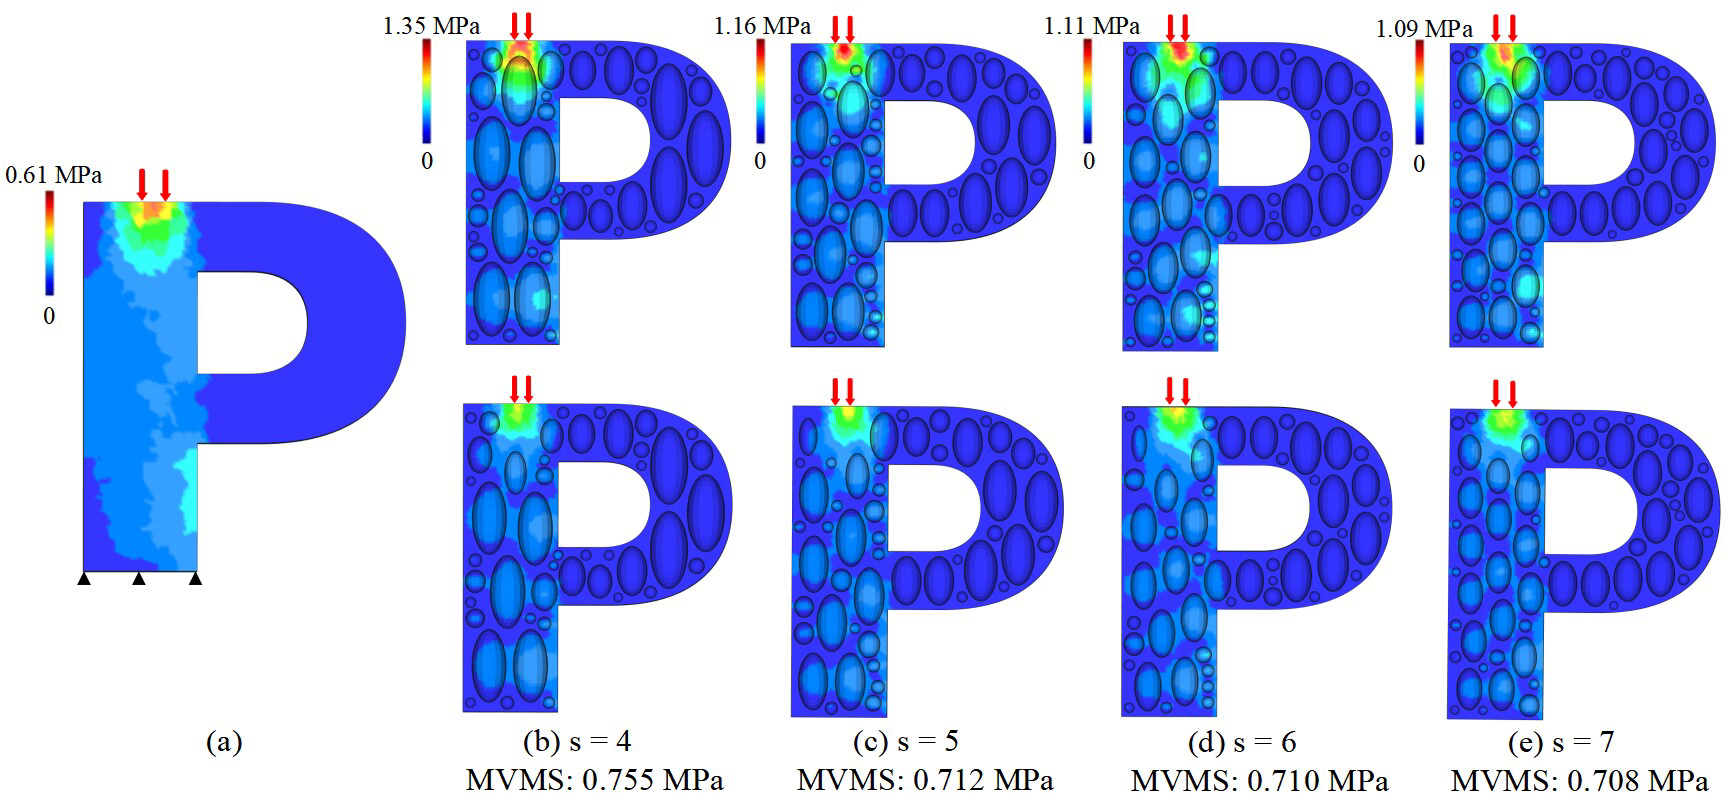
\includegraphics[width=1.0 \textwidth]{./figures/self-support/fig7.png}
  \caption{尺寸参数 $s$ 的影响}
  \label{fig:6}
\end{figure*}
优化的主要目标是在满足目标体积约束的前提下,提高结构的物理性能,而非仅关注实现自支撑特性。结构的自支撑特性在初始化阶段即已确立,在优化过程中,通过限制主半径最大范围来确保自支撑能力,该方法有助于减少优化过程中的约束条件数量。

\paragraph{问题的离散化。}
与传统有限元分析不同,每次迭代都需要对四面体或六面体网格进行重网格化来描述形状并计算,而重网格化过程非常耗时,且容易出现网格失败或质量较差的问题。在本章方法中,形状由连续函数描述,仅需构建一次统一的有限六面体单元作为积分域,并在整个优化过程中保持六面体单元不变。方程~\ref{eq:7}中的优化问题可重写为离散形式,
\begin{equation}
\centering
    \begin{split}
        \min \quad & I = U^{T} K U,   \\
        s.t. \quad & K U = F,       \\
        &V = \frac{1}{8}\sum _{i=1}^{n} \sum _{j=1}^{8}G(\overline{\phi}_{i,j})- \sum _{k=1}^{n_{e}} \frac{4}{3} \pi a_{k} b_{k} c_{k} \leq V_{c}, \\
        &\sum _{i=1}^{n_{e}} \sum _{j=1}^{n_{e}-1}E_{s}^{ij}=0, 
    \end{split}
    \label{eq:9}
\end{equation}
其中$U$是位移矩阵,$F$是体力向量,$n$是用于积分计算的离散单元数量,$n_{e}$是椭球体空腔的数量,$V_{c}$是体积约束,$\overline{\phi}{i,j}$是第$i$个单元的第$j$个节点点处$\overline{\phi}(*)$的值,$K$是刚度矩阵,其中$K_i$是第$i$个单元的刚度矩阵,($a_k$,$b_k$,$c_k$)是第$k$个椭球体的三个主半径,$E{s}^{ij}$是第$i$个椭球体与第$j$个椭球体之间的碰撞检测。

\subsection{优化求解过程}
良好的初始化有助于加快优化收敛,本节提供了一种基于输入模型结构强度构建的应力初始化方法。给定均匀采样的椭球体质心,目标是获得一个无交叉的自支撑椭球体填充。根据公式 (\ref{eq:1}) 中的自支撑计算,仅需获得每个椭球体的主半径$c$,其他两个主半径$a$和$b$的最大值可以推导得出。第$i$个椭球体的主半径$c_i$可计算为
\begin{equation}
  c_{i} = e^{-{(2\sigma_{n}})^2}*\frac{h_{max}}{s},
  \label{eq:6}
\end{equation}
其中,$\sigma_n$为标准化结构应力,$h_{max}$为输入模型最大高度,$s$为调整自支撑椭球体大小和数量的缩放因子。缩放因子$s$影响椭球体空腔大小和数量,但对优化结构力学性能影响较小。在相同填充比下,缩放因子$s$越大,椭球体空腔数量越多。当缩放因子$s$取6时,在结构强度和椭球体数量间达到了良好平衡,如图~\ref{fig:6}所示。获得椭球体初始主半径后,将使用自动定位检测调整椭球体大小。当无相交椭球体时,即可获得初始化。


$n_e$个椭球体的变量包括主半径${(a_i,b_i,c_i)}{i=1}^{n_e}$和中心点${(x_i,y_i,z_i)}{i=1}^{n_e}$。在优化过程中,如果未施加限制,椭球体很可能发生碰撞,这种碰撞会损害结构的自支撑性能。为解决这一问题,可采用GJK算法~\cite{gilbert1988fast}检测椭球体间碰撞,并计算每个椭球体的可行运动范围,确保无碰撞运动。

为避免优化迭代中椭球体频繁碰撞,设置了设计变量上限,将椭球体限制在各自可行范围内。然而,在每次迭代中重新计算每个椭球体可行范围会带来大量额外计算开销。实际上,无需在单次迭代中求解所有椭球体可行范围。大多数椭球体在优化过程中保持不变,无需进行碰撞检测。通过排除这些不变椭球体,可提高计算效率,并保持优化问题可微分性。剩余的被称为关键椭球体的,是根据上次迭代梯度值确定的。在迭代过程中,仅监测涉及关键椭球体的碰撞。初始时通常仅有少数关键椭球体,在优化过程中数量逐渐增加,但相对保持较小。

每步迭代, 形状参数 $\{(a_i,b_i,c_i)\}^{n_e}_{i=1}$ 首先被优化,局部参数 $\{(x_i,y_i,z_i)\}^{n_e}_{i=1}$ 先固定。目标函数关于变量的梯度可以计算得到:
\begin{equation}
  \begin{split}
      &\frac{\partial I}{\partial t_{k}} =-U^T\frac{\partial K}{\partial t_{k}}U=-U^T[{\frac{1}{8}}\sum_{i=1}^{n} \sum_{j=1}^{8}q(G(\phi^{o}_{ij}))^{q-1}\frac{\partial {G(\phi^{o}_{ij})}}{\partial t_{k}}K_{i}]U,               \\
      &\frac{\partial V}{\partial t_{k}} = \sum_{k=1}^{n_{e}} \frac{4}{3} \pi \frac{a_{k}b_{k}c_{k}}{t_{k}},  \ \\
      &\frac{\partial G(\phi^{o}_{ij})}{\partial t_{k}} = \frac{\partial G}{\partial \phi^{o}_{ij}} \dot \frac{\partial \phi^{o}_{ij}}{\partial t_{k}}, 
  \end{split}
\end{equation}
其中,$t_k$表示待优化参数,可以采用移动渐近线优化器~\cite{svanberg1987method}中的相应$\partial I / \partial t_{k}$来更新形状参数${(a_i,b_i,c_i)}_{i=1}^{n_e}$。如果某个椭球体更新后的形状参数最小值低于第3.1节提到的指定阈值,则将其移除,并将椭球体数量更新为$n_e=n_e-1$。
接下来,采用类似的方法优化位置参数${(x_i,y_i,z_i)}_{i=1}^{n_e}$,同时保持更新后的形状参数固定不变。
尽管无法通过数学推导保证收敛,但在实验中,所有结果都在数十次迭代内收敛。

\begin{figure*}[htbp]
  \begin {center}
  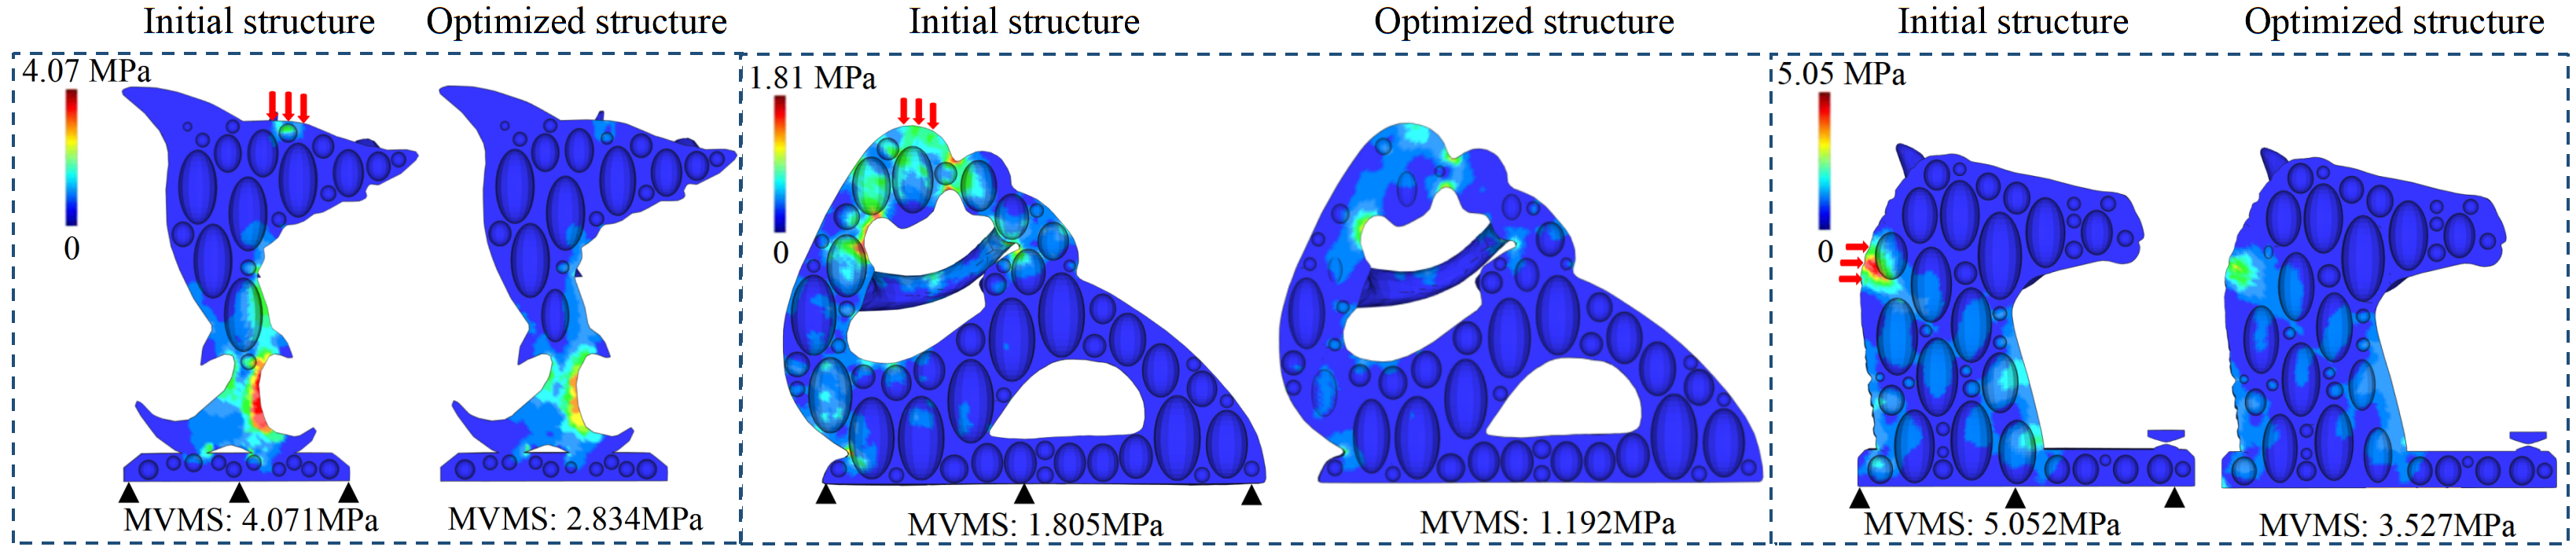
\includegraphics[width=0.98 \textwidth]{./figures/self-support/fig8.png}
  \caption{初始结构和优化结构的应力分布比较}
  \label{fig:7}
  \end {center}
\end{figure*}

\begin{figure}[htbp]
  \begin {center}
  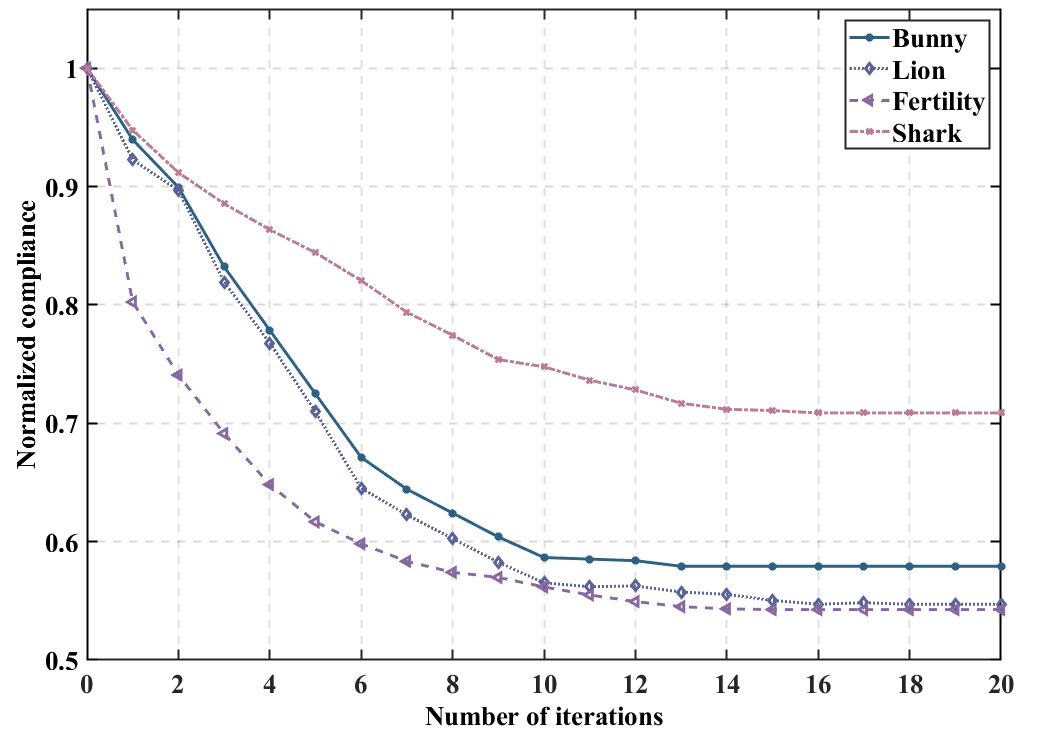
\includegraphics[width=0.6 \linewidth]{./figures/self-support/fig9.png}
  \caption{四个模型的收敛曲线}
  \label{fig:8}
  \end {center}
\end{figure}

\section{实验和讨论}
本节测试了所提出的自支撑空心化方法在各个方面的性能。默认情况下,在固定底部的情况下,在顶部施加1.0 $N/mm^2$的表面压力。填充的自支撑结构由3D打印机使用0.2 mm的切片厚度和弹性模量为3000 MPa、泊松比为0.35的PLA塑料打印。
设计和优化过程中涉及一些参数,其中大部分参数与模型无关,可以默认固定。所有实验均在一台配备3.70GHz Intel(R)Core(TM) i9-10900 CPU和128 GB RAM的计算机上进行。

\begin{figure}[htbp]
  \begin {center}
  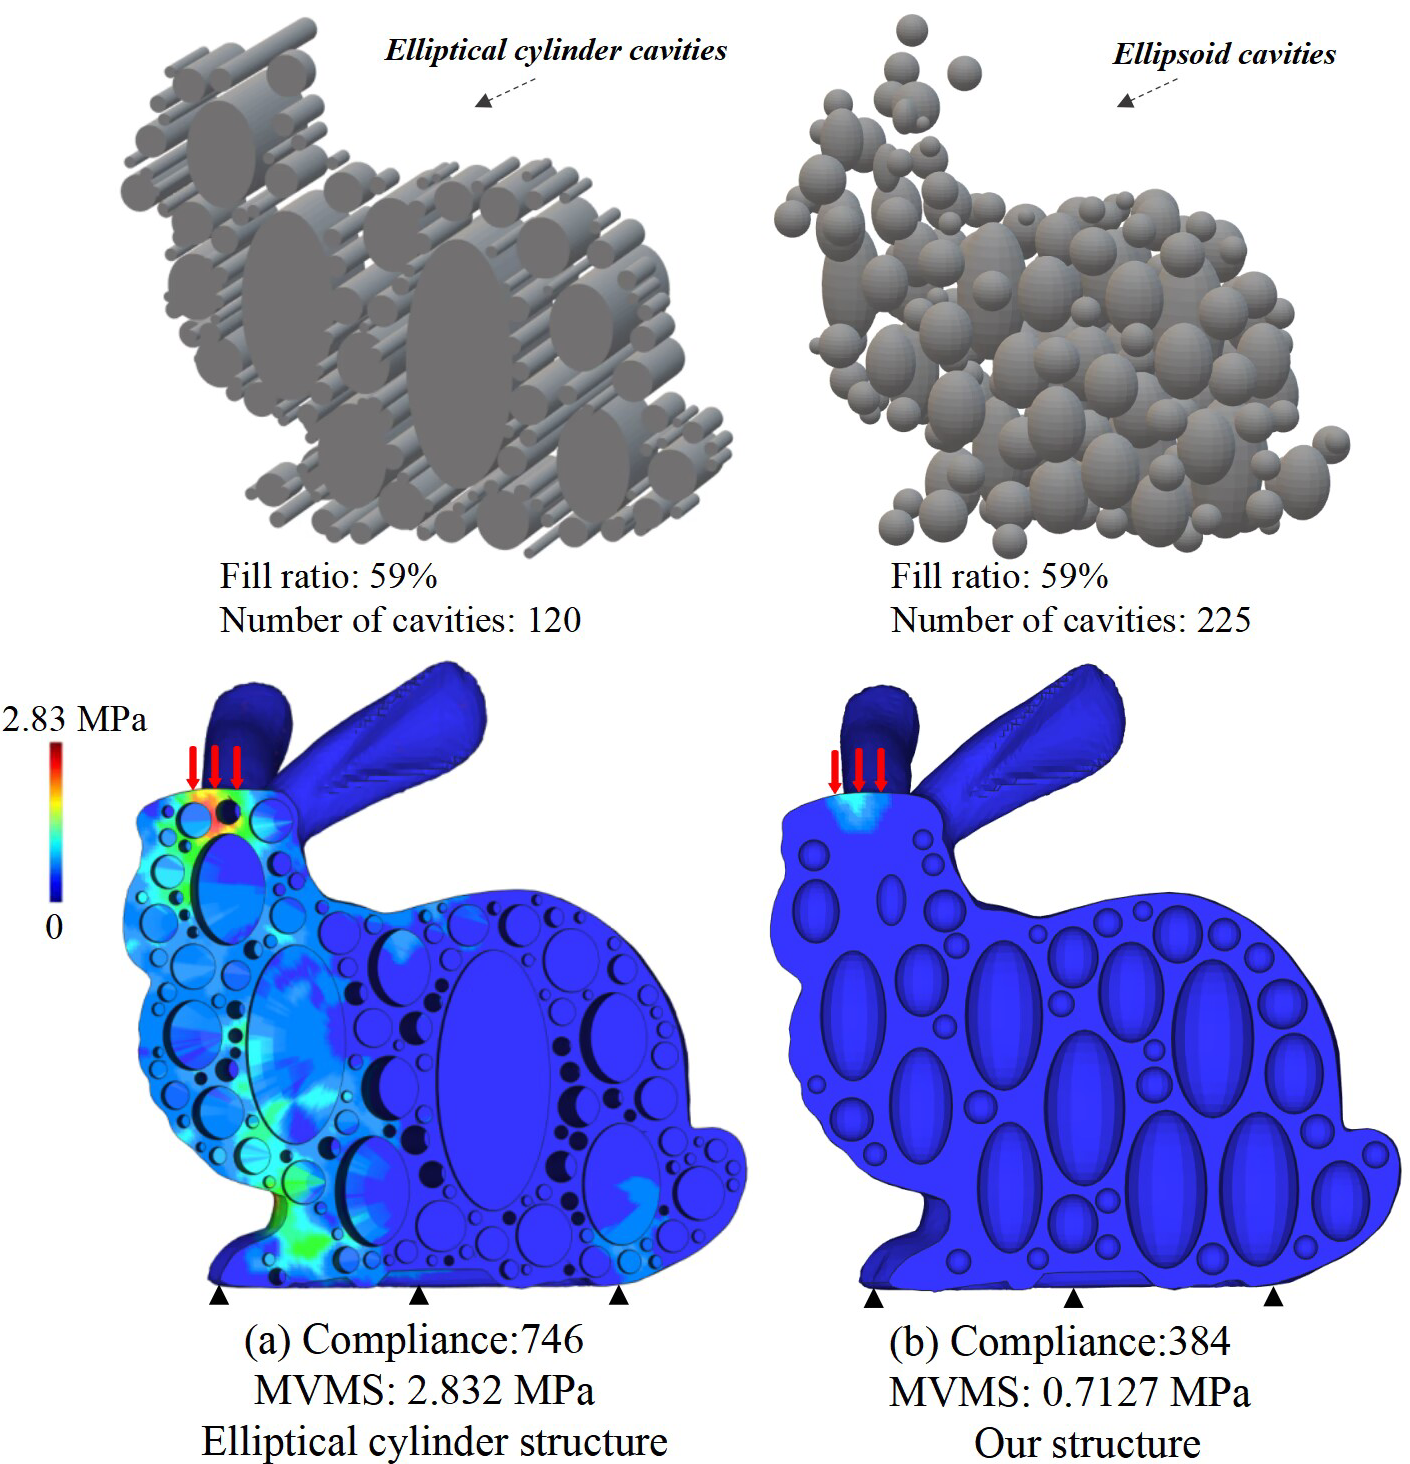
\includegraphics[width=0.65 \textwidth]{./figures/self-support/fig10.png}
  \caption{与椭圆柱体结构方法 \cite{lee2018support} 在相同填充比例下的比较实验 }
  \label{fig:9}
  \end {center}
\end{figure}

\subsection{有效性和效率性}
众所周知,在基于传统有限元分析(FEA)的优化方法中,生成四面体网格和/或六面体网格需要耗费大量时间。而且在传统基于FEM的优化过程中,重新网格化是必需的步骤,用于表示形状并执行计算。
相比之下,基于函数的3D模型表示方法可以直接在离散计算中对这些函数进行积分和梯度计算,仅需构建一次简单的均匀有限元作为积分域即可。在建模和优化过程中不需要频繁重新网格化,这导致数值计算非常高效和稳定,特别是对于大型复杂结构。
图~\ref{fig:7}显示了初始化和相应的优化结果。所提出的方法生成了轻量级且强度高的模型,这些模型通过优化的自支撑椭球体进行了空心化,并具有良好的力学性能。相应模型的时间和优化数据如表~\ref{T:table1}所示。在几何(形状和位置)和拓扑(空腔数量)优化后,最大冯·米塞斯应力(MVMS)得到了显著改善。
使用传统有限元分析很难获得优化的椭球体,这里仅列出了FEA中一次迭代的计算时间。所提出的方法更加高效,所有实验都在数十步内收敛,总时间(包括初始化和优化)每个模型不到一小时。

此外,所提出的基于函数的框架提供了精确的解析梯度,并确保了优化的数值稳定性。图~\ref{fig:8}展示了四种不同模型的收敛曲线。为了直观显示,收敛曲线已经通过刚度能量进行了归一化处理,这些模型均在20次迭代内实现了收敛。


\begin{table*}
    \centering
    \fontsize{7.5}{8}\selectfont
    \caption{实验结果表:优化数据和时间 }
    \label{T:table1}
    % Please add the following required packages to your document preamble:
    % \usepackage{multirow}
    \renewcommand{\arraystretch}{1.5}
    \setlength{\tabcolsep}{1.2mm}{
    \resizebox{1.0\linewidth}{!}{
        \begin{tabular}{c|ccc|ccc|cc|c|clllll}
            \cline{1-11}
            \multirow{2}{*}{\textbf{模型}} & \multicolumn{3}{c|}{\textbf{初始空心化模型}} & \multicolumn{3}{c|}{\textbf{优化空心化模型}} & \multicolumn{2}{c|}{\textbf{优化}} & \multirow{2}{*}{\textbf{总时间}(min)} & \multirow{2}{*}{\textbf{一步FEA时间}(min)} & \multicolumn{2}{c}{} & \multicolumn{1}{c}{}          & \multicolumn{1}{c}{\multirow{2}{*}{}} & \multicolumn{1}{c}{\multirow{2}{*}{}}                                                                                   \\ \cline{2-9}
                                   & \multicolumn{1}{c}{MVMS(MPa)}             & \multicolumn{1}{c}{\# Ellipsoids}           & Fill ratio                        & \multicolumn{1}{c}{MVMS(MPa)}    & \multicolumn{1}{c}{\# Ellipsoids}  & Fill ratio           & \multicolumn{1}{c}{Time(min)} & \#iterations                          &                                       &      & \multicolumn{1}{c}{} &  &  & \multicolumn{1}{c}{} & \multicolumn{1}{c}{} \\ \cline{1-11}
            P                      & \multicolumn{1}{c}{1.11}                  & \multicolumn{1}{c}{228}                     & 55.6\%                            & \multicolumn{1}{c}{0.71}         & \multicolumn{1}{c}{219}            & 59.47\%              & \multicolumn{1}{c}{2.31}      & 20                                    & 52.6                                  & 4.22 &                      &  &  &                      &                      \\
            Bunny                  & \multicolumn{1}{c}{1.49}                  & \multicolumn{1}{c}{231}                     & 54.21\%                           & \multicolumn{1}{c}{0.713}        & \multicolumn{1}{c}{225}            & 59.03\%              & \multicolumn{1}{c}{2.26}      & 16                                    & 46.2                                  & 3.67 &                      &  &  &                      &                      \\
            Shark                  & \multicolumn{1}{c}{4.07}                  & \multicolumn{1}{c}{213}                     & 62.31\%                           & \multicolumn{1}{c}{2.83}         & \multicolumn{1}{c}{208}            & 65.02\%              & \multicolumn{1}{c}{2.24}      & 17                                    & 42.6                                  & 3.18 &                      &  &  &                      &                      \\
            Fertility              & \multicolumn{1}{c}{1.81}                  & \multicolumn{1}{c}{193}                     & 59.42\%                           & \multicolumn{1}{c}{1.19}         & \multicolumn{1}{c}{183}            & 64.98\%              & \multicolumn{1}{c}{2.21}      & 16                                    & 41.4                                  & 3.25 &                      &  &  &                      &                      \\
            Molar                  & \multicolumn{1}{c}{8.92}                  & \multicolumn{1}{c}{330}                     & 50.54\%                           & \multicolumn{1}{c}{5.94}         & \multicolumn{1}{c}{329}            & 55.81\%              & \multicolumn{1}{c}{2.37}      & 18                                    & 53.9                                  & 3.75 &                      &  &  &                      &                      \\
            Kitten                 & \multicolumn{1}{c}{2.58}                  & \multicolumn{1}{c}{413}                     & 42.27\%                           & \multicolumn{1}{c}{1.59}         & \multicolumn{1}{c}{402}            & 54.48\%              & \multicolumn{1}{c}{2.41}      & 18                                    & 52.2                                  & 4.03 &                      &  &  &                      &                      \\

            Horse                  & \multicolumn{1}{c}{5.05}                  & \multicolumn{1}{c}{567}                     & 38.42\%                           & \multicolumn{1}{c}{3.51}         & \multicolumn{1}{c}{564}            & 41.5\%               & \multicolumn{1}{c}{2.54}      & 16                                    & 46.7                                  & 3.53 &                      &  &  &                      &                      \\ \cline{1-11}
        \end{tabular}}}
\end{table*}


\subsection{比较和讨论}
为验证所提出方法的有效性,结果与最相关的椭圆柱结构~\cite{lee2018support}进行了比较。
椭圆柱方法使用贪心初始化生成空腔结构,但无法优化相应结构。此外,椭圆柱结构由2D椭圆拉伸而成,在具有复杂几何和拓扑的形状中会出现空心化问题。所提出的椭球体在3D空间中构建,具有更高的自由度,轴长和位置可以使用高效的无网格方法进行优化。优化后的结构明显优于~\cite{lee2018support}方法的结果。
柔度反映了整体结构强度,最大冯·米塞斯应力(MVMS)用于反映结构中最薄弱的局部区域。结构柔度或MVMS越小,结构越强。
如图~\ref{fig:9}所示,椭圆柱结构和所提出结构的顺应性分别为746和384,两种结构的MVMS分别为2.832 MPa和0.7127 MPa。这表明,在相同条件(外载和体积约束)下,所提出结构的刚度明显优于椭圆柱结构。

本文还与与其他相关方法进行了比较,包括菱形结构~\cite{wu2016self}、三角-六边形结构~\cite{xu2021support}、基于TPMS的结构~\cite{hu2020efficient}和蜂窝结构~\cite{10.1145/2601097.2601168},所有模型在相同外载下进行了测试。
图~\ref{fig:10} (a)-(d)展示了在相同54.5\%填充比下,菱形结构(a)、三角-六边形结构(b)和所提出结构(c)的比较。相应的最大冯·米塞斯应力(MVMS)分别为3.615 MPa、3.512 MPa和1.589 MPa。本文方法所优化结构的MVMS更接近于实心模型(d),各结构的柔度值分别为1194、1169、760和512。
菱形结构通过细分初始菱形单元自适应构建,可优化变量仅为细分层级,自由度小于所提出方法。三角-六边形结构具有良好刚度,但未对结构进行优化。
\begin{figure*}[htbp]
    \begin {center}
    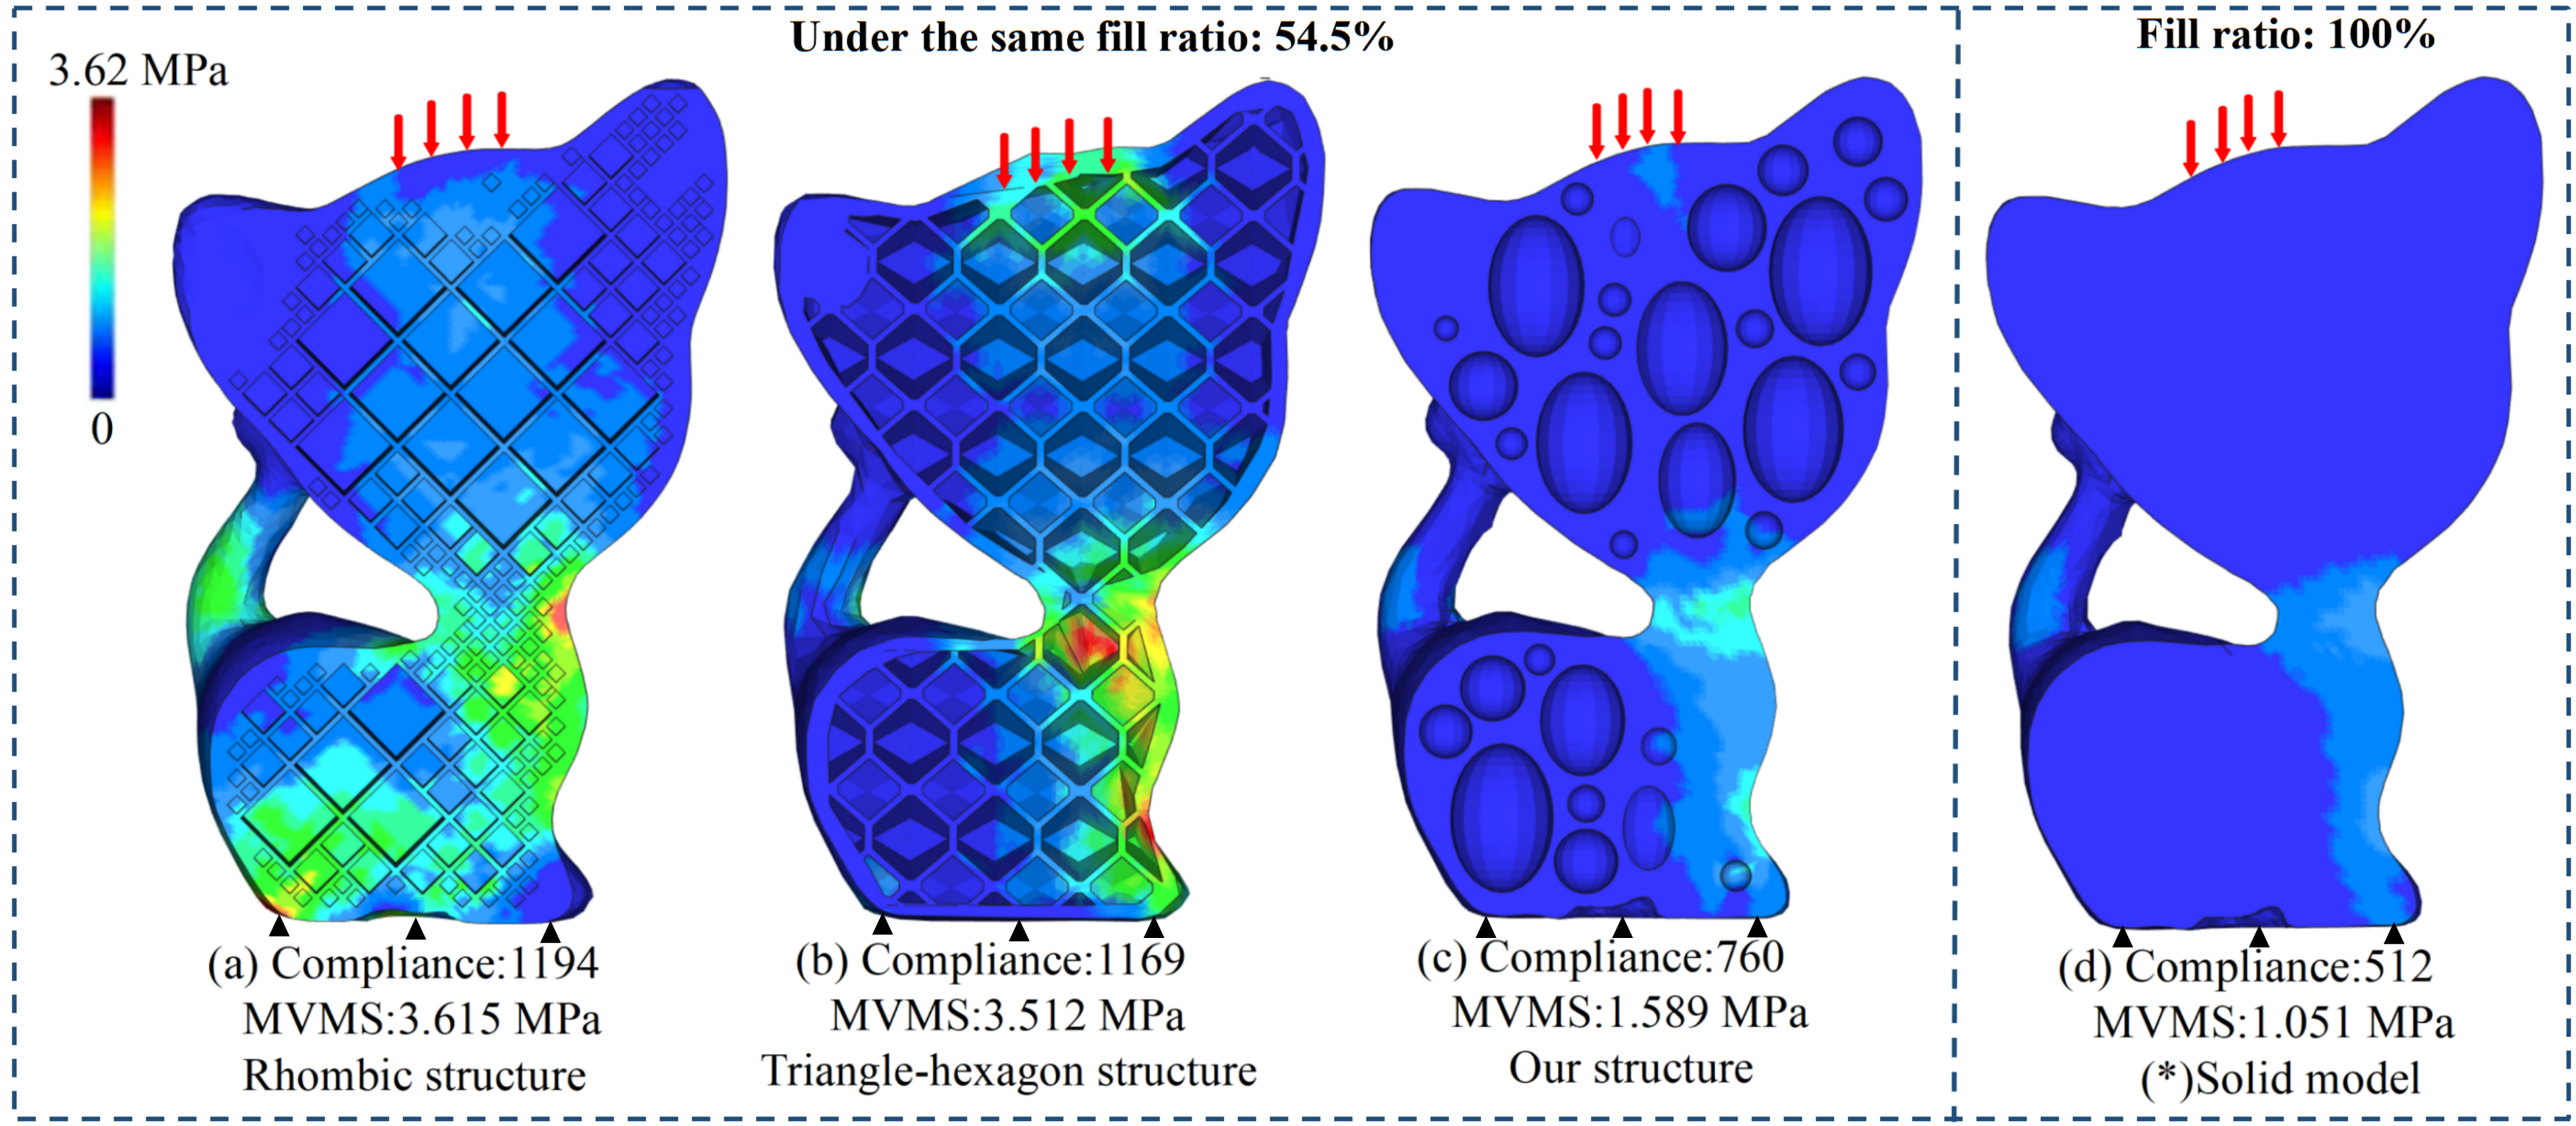
\includegraphics[width=0.8 \textwidth]{./figures/self-support/fig11.png}
    \caption{与相关自支撑空心轻量化方法的比较~\cite{wu2016self,xu2021support}}
    \label{fig:10}
    \end {center}
\end{figure*}

本文方法还与一些非自支撑结构进行了比较,包括蜂窝结构~\cite{10.1145/2601097.2601168}和基于TPMS的结构~\cite{hu2020efficient},如图~\ref{fig:11}所示。
蜂窝结构通过启发式算法进行优化,需要在每次迭代中进行耗时的重网格化。相比之下,所提出的结构可以通过函数进行表示、设计和优化,有利于数值计算的稳定性和快速收敛。
基于TPMS的结构可以使用连续表示自动优化,但由于受TPMS构造的限制,该结构在狭窄和薄弱部位容易出现脆弱性。
比较结果表明,所提出的自支撑结构刚度优于其他结构。主要原因是,该自支撑结构可以直接在函数上进行解析计算,并具有更多可优化的自由度,包括形状(椭球体尺寸)、位置(椭球体位置)和拓扑(椭球体数量)。
在相同45.3\%的填充比下,所提出结构的MVMS和填充比更接近于实心模型(填充比100\%)。
为了更清晰地说明,图~\ref{fig:14}中绘制了这些方法的MVMS直方图。直方图清楚地显示,所提出的结果具有最佳性能,与实心模型相当。
上述相关方法的总结列于表~\ref{T:table2}中。该方法在自支撑性、强度导向性、表示、优化和可优化自由度等方面具有明显优势。

\begin{figure*}[b]
    \begin {center}
    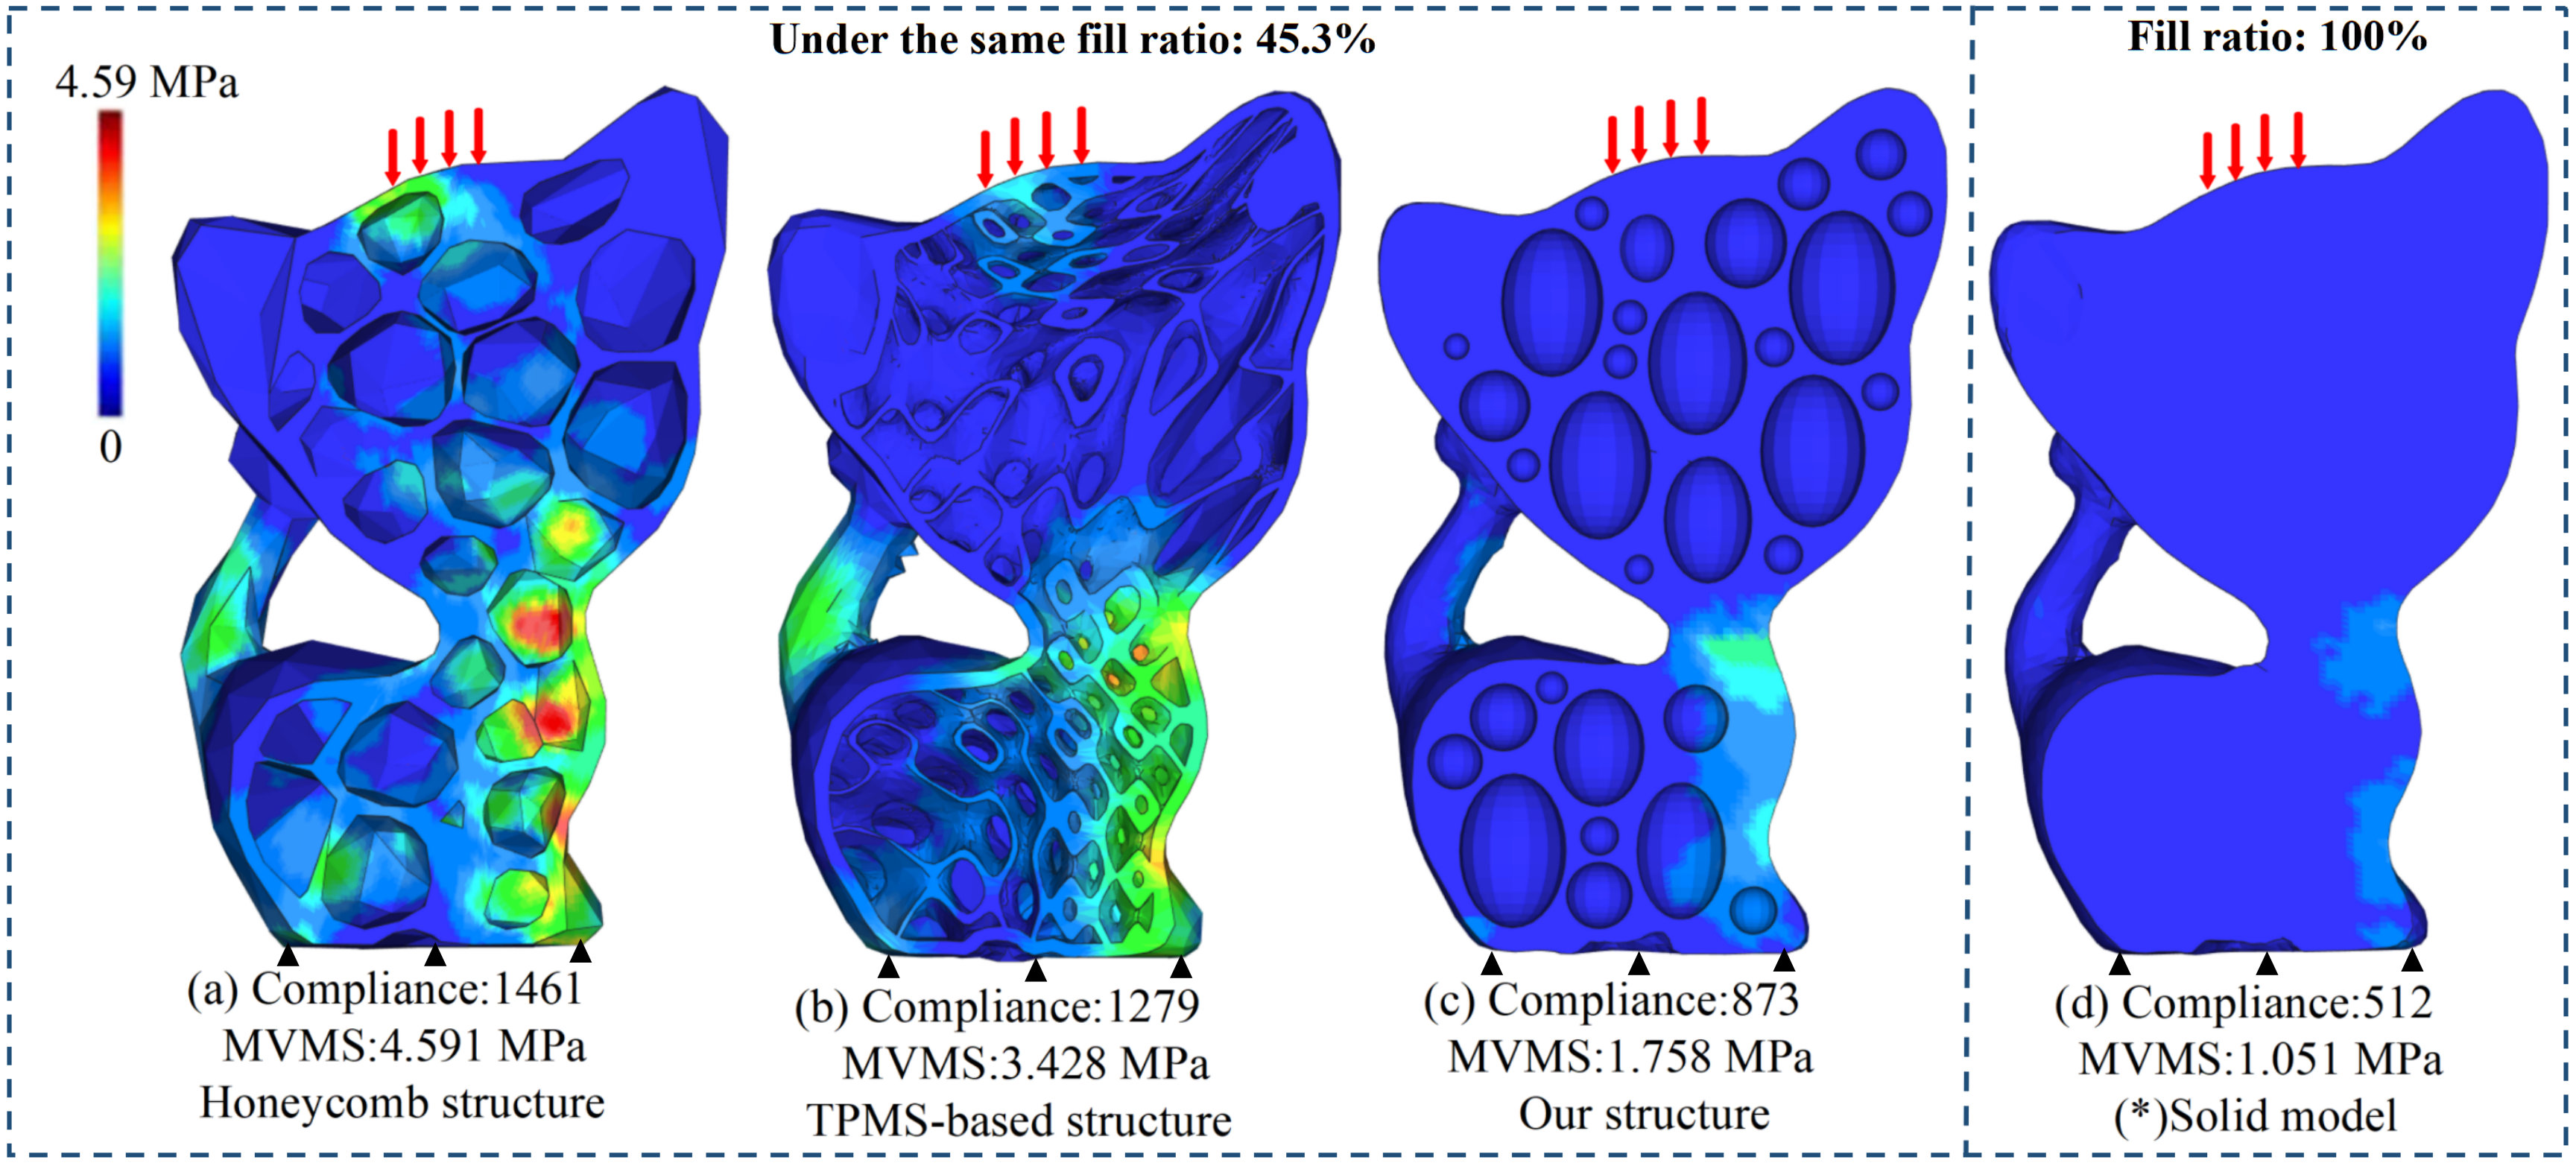
\includegraphics[width=0.8 \textwidth]{./figures/self-support/fig12.png}
    \caption{与相关非自支撑轻量化方法~\cite{10.1145/2601097.2601168,hu2020efficient}的比较}
    \label{fig:11}
    \end {center}
\end{figure*}

\begin{table*}[htbp]
  \centering
  \centering
  \fontsize{7}{8}\selectfont
  \caption{相关方法的定性比较}
  \label{T:table2}
  \renewcommand{\arraystretch}{1.5}
  \setlength{\tabcolsep}{1.8mm}{
  \resizebox{1.0\linewidth}{!}{
      \begin{tabular}{c|c|c|c|c|c}
          \toprule
          \textbf{方法}                                    & \textbf{自支撑性}     & \textbf{强度优化}   & \textbf{表示方法}      & \textbf{优化形式}       & \textbf{优化自由度}         \\ 
          \midrule
          Honeycomb structures in \cite{10.1145/2601097.2601168}      & ×                   & \checkmark          & 离散            & 启发式          & 3D (几何+拓扑)                   \\
          Rhombic structures in \cite{wu2016self}                     & \checkmark          & \checkmark          & 离散            & 自动          & 3D (几何+拓扑)
          \\
          Support-free hollowing structures in \cite{wang2018support} & \checkmark          & ×                   & 离散            & none               & none
          \\
          Elliptical cylinder structures in \cite{lee2018support}     & \checkmark          & ×                   & 离散            & none               & none                                  \\
          TPMS-based structures in \cite{hu2020efficient}             & ×                   & \checkmark          & 连续           & 自动          & 3D (几何+拓扑)                   \\
          Triangle-hexagon structures in \cite{xu2021support}         & \checkmark          & \checkmark          & 离散            & none               & none                                  \\
          \midrule
          \textbf{本文方法}                                        & \textbf{\checkmark} & \textbf{\checkmark} & \textbf{连续} & \textbf{自动} & \textbf{3D (几何+位置+拓扑)} \\ 
          \bottomrule
      \end{tabular}}}
\end{table*}

\begin{figure}[htbp]
  \begin {center}
  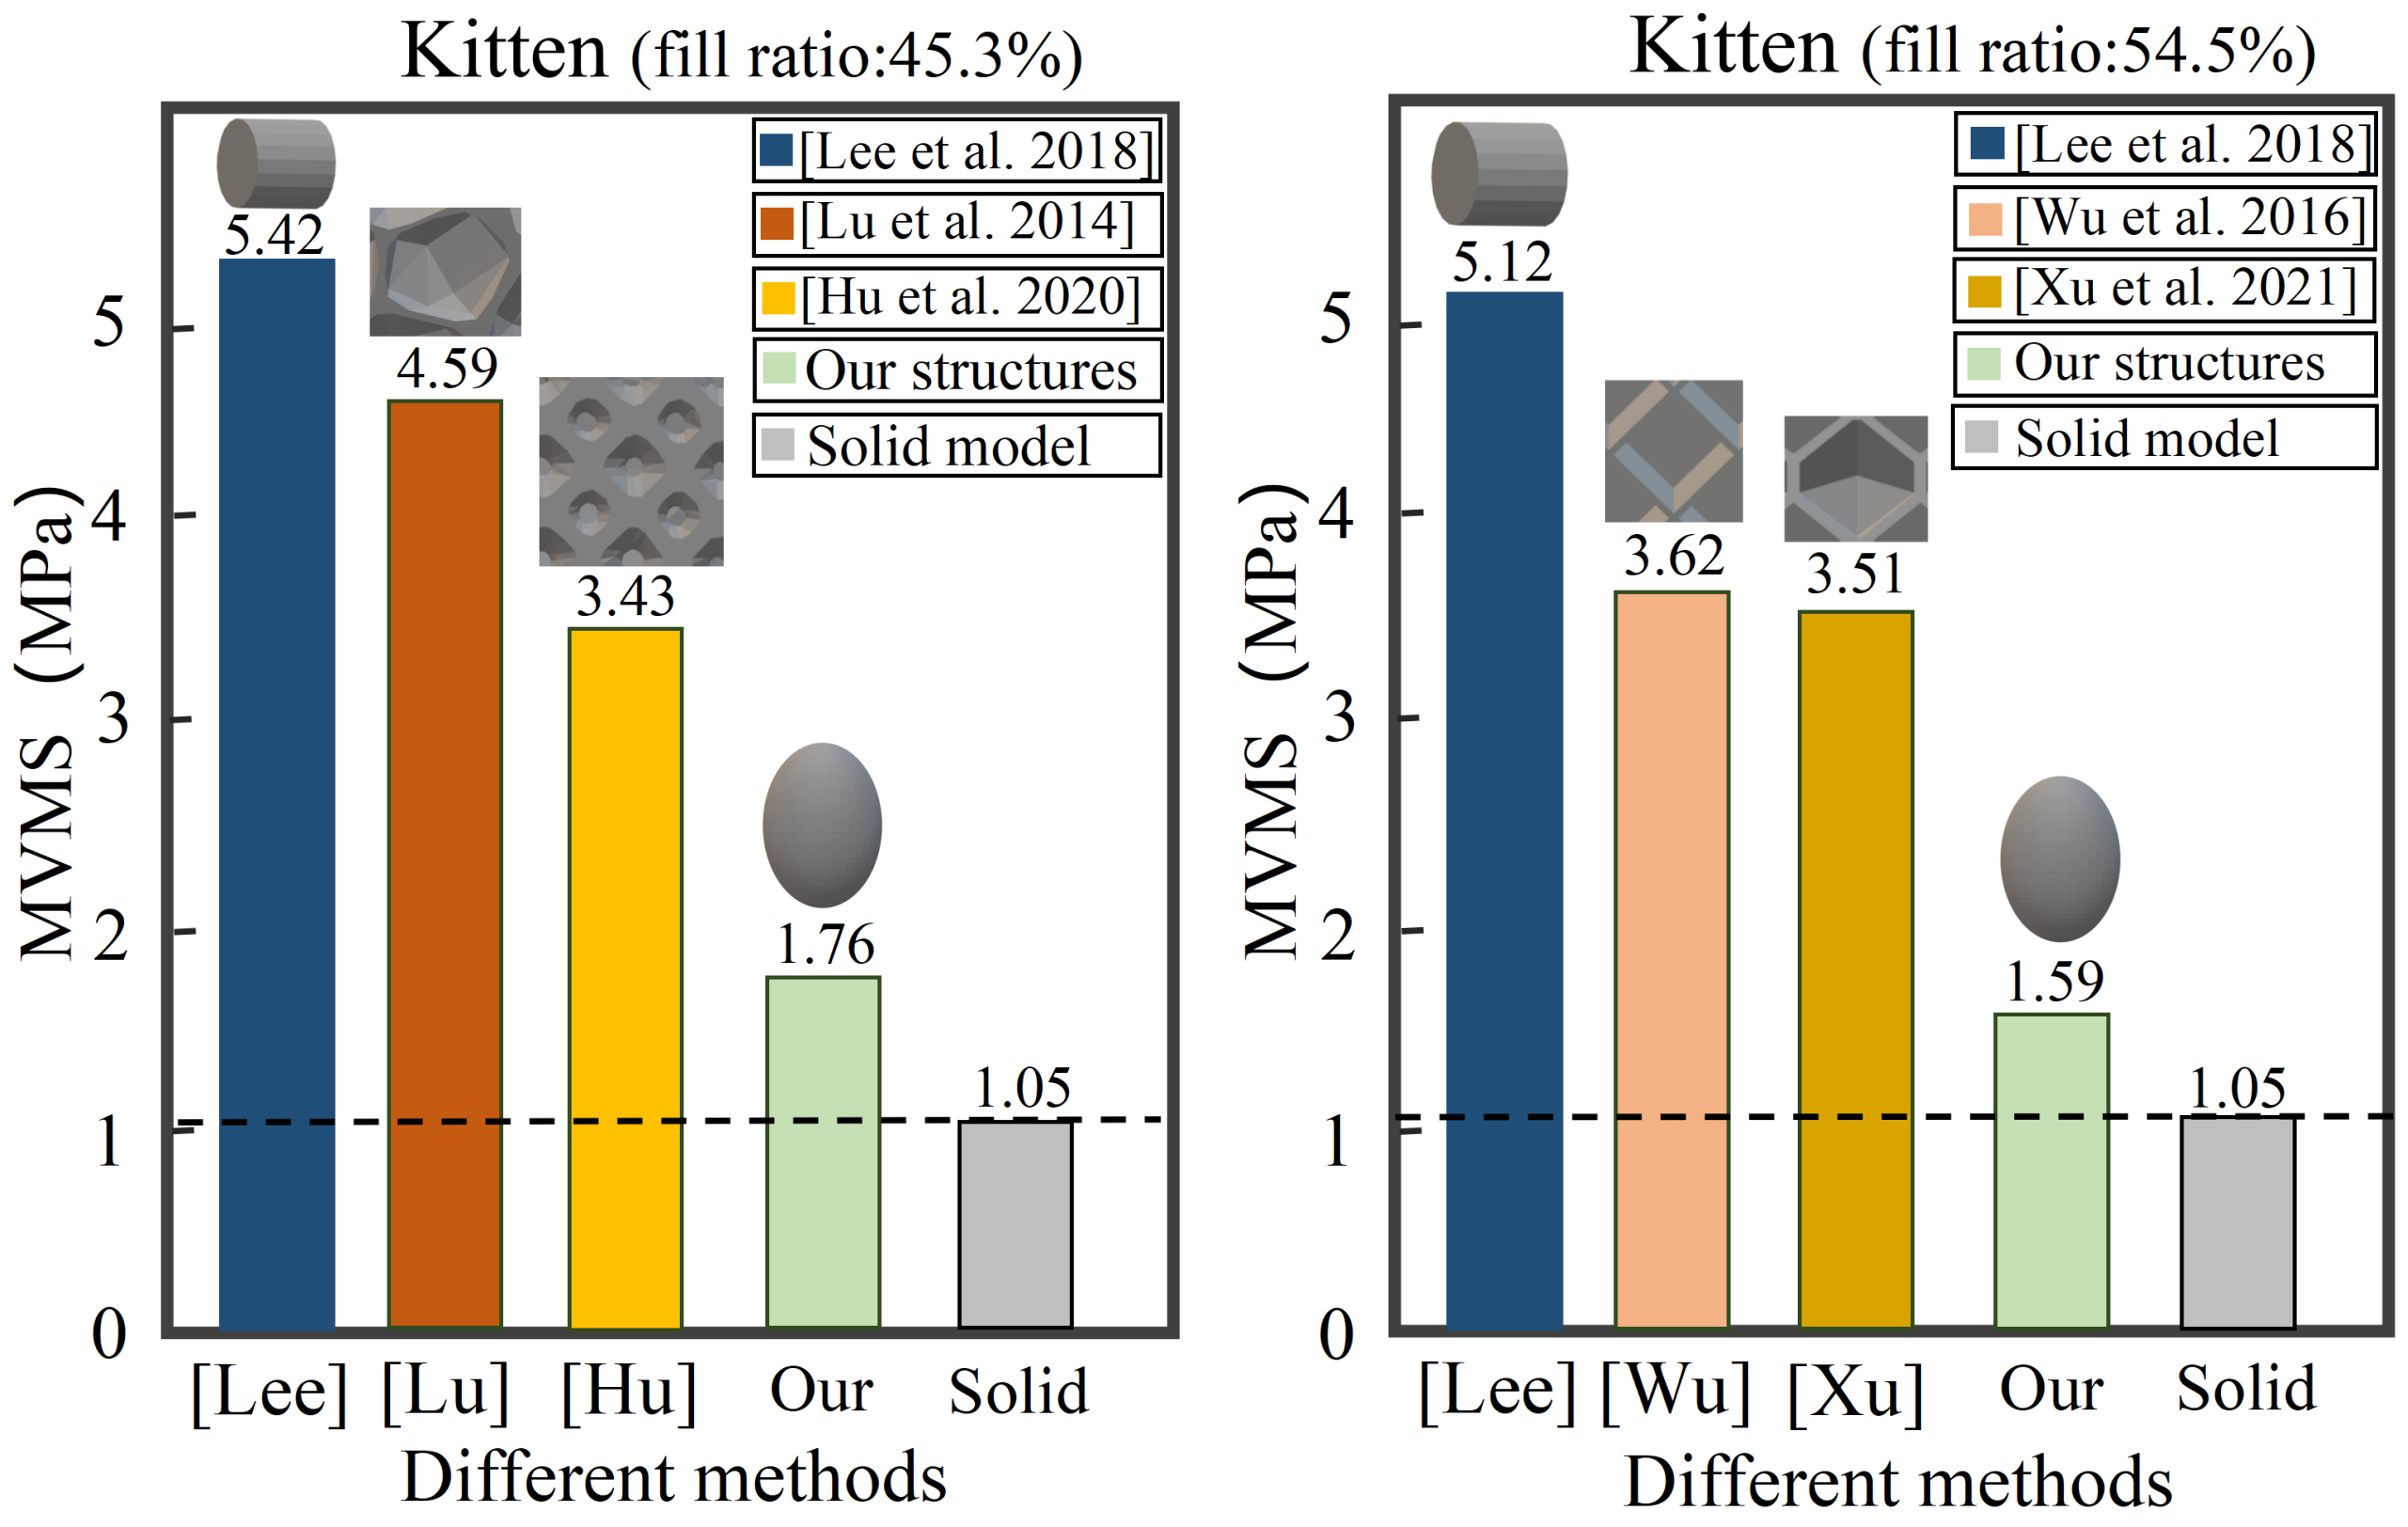
\includegraphics[width=0.8 \textwidth]{./figures/self-support/fig14.png}
  \caption{相同填充比例下不同方法\cite{xu2021support,10.1145/2601097.2601168,wu2016self,hu2020efficient}的MVMS比较直方图}
  % \caption{Histograms of MVMS under the same fill ratio (left:45.3$\%$, right:54.5$\%$). Our structures have the smallest MVMS among the related methods, including
  %     the elliptical cylinder structure \cite{lee2018support},
  %     the Triangle-hexagon structure \cite{xu2021support},
  %     the Honeycomb structure \cite{10.1145/2601097.2601168},
  %     the Rhombic structure \cite{wu2016self} and
  %     the TPMS-based structure \cite{hu2020efficient}.
  %     Our structures are comparable to the solid model.}
  \label{fig:14}
  \end {center}
\end{figure}

\begin{figure}[htbp]
  \begin {center}
  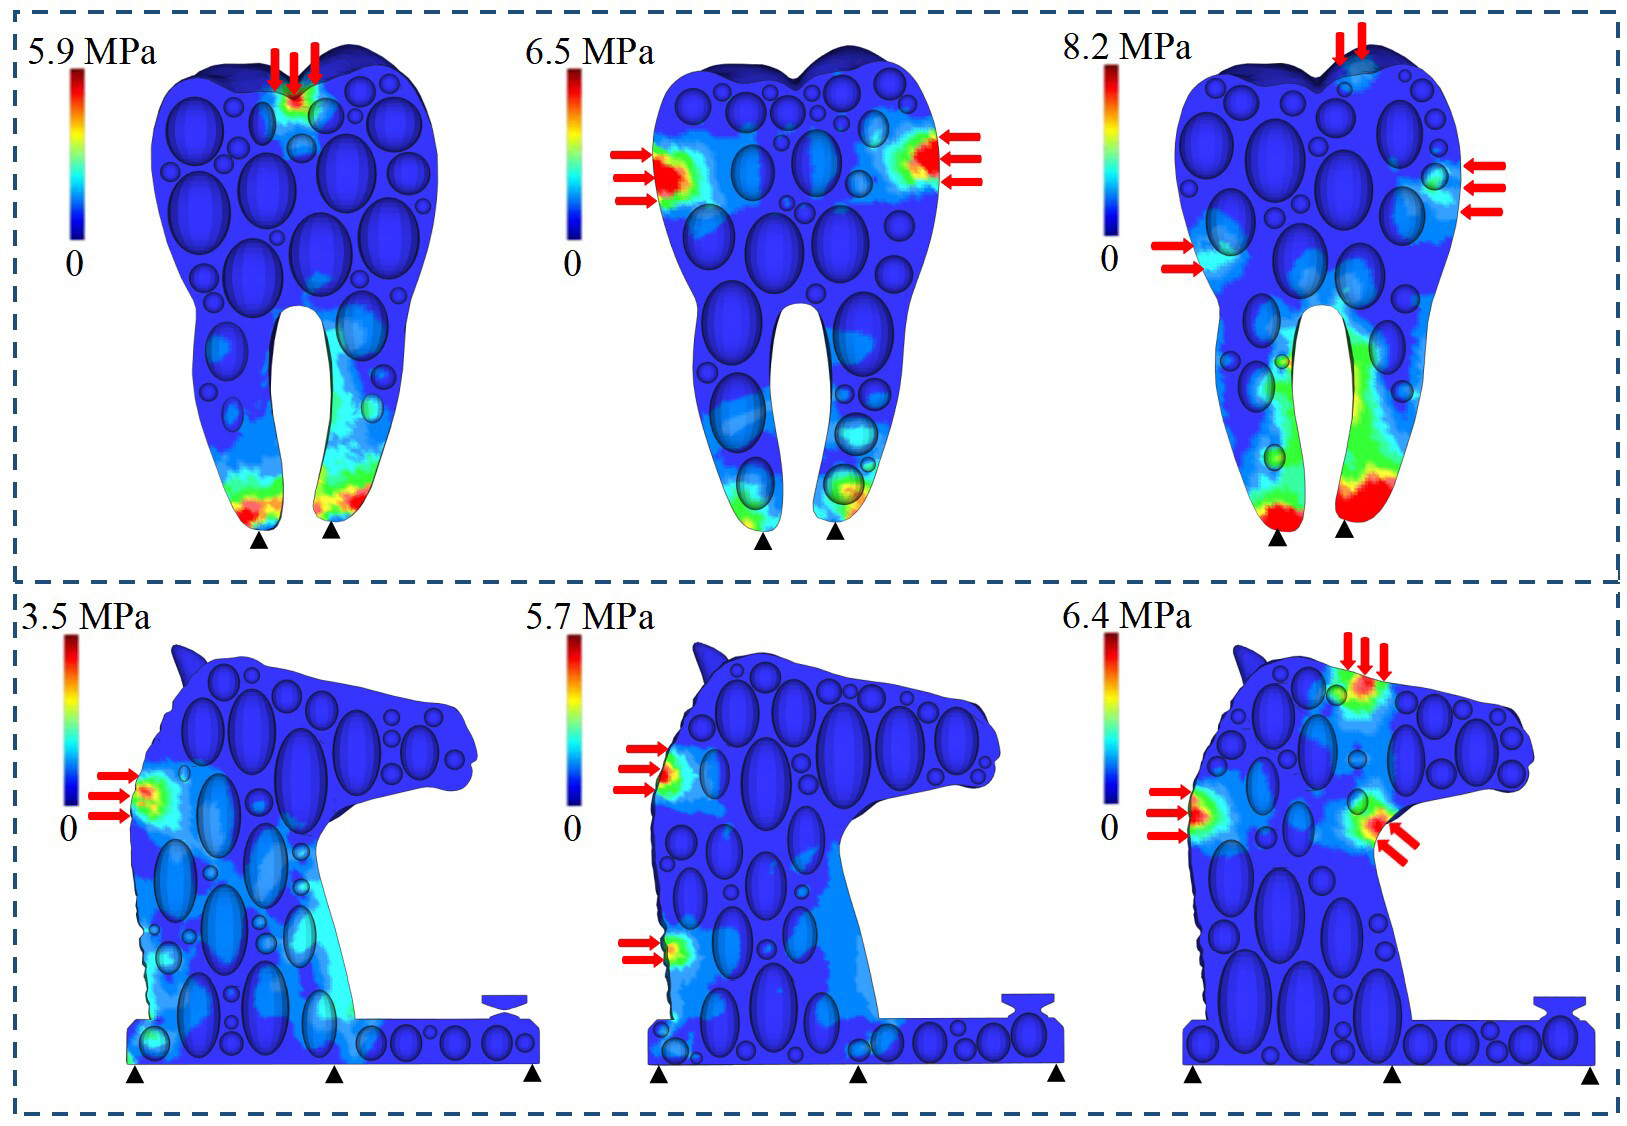
\includegraphics[width=0.9 \textwidth]{./figures/self-support/fig13.png}
  \caption{不同受力方向下的优化结构}
  \label{fig12}
  \end {center}
\end{figure}
所提出的框架支持多种载荷工况。为验证该方法在不同载荷条件下的有效性,如图~\ref{fig12}所示,对其进行了进一步测试。在不同工况下,该方法表现良好,并获得了给定载荷条件下的最优结构。
外力方向没有限制,与椭球体或制造方向无关。
该方法采用的椭球体为各向异性孔隙,当其与应力方向一致时,其机械性能优于等向孔隙。
此外,优化后的模型可通过常见的FDM 3D打印技术制造。
为评估可行性,如图~\ref{fig:15}所示,使用FDM 3D打印机打印了几个优化后的模型。在所有实验中,内部结构均可良好打印,无需额外支撑。
此外,如图~\ref{fig:16}所示,使用RG1-5微型计算机控制电子万能试验机对3D打印模型进行了测试,该结构的机械性能与实心模型相当。两种模型在高荷载下都保持良好状态,即使试验机达到最大5000N的力,主体结构仍然完好。
因此,所提出的方法得到的优化结构是可信和可行的。

\begin{figure*}[htbp]
  \begin {center}
  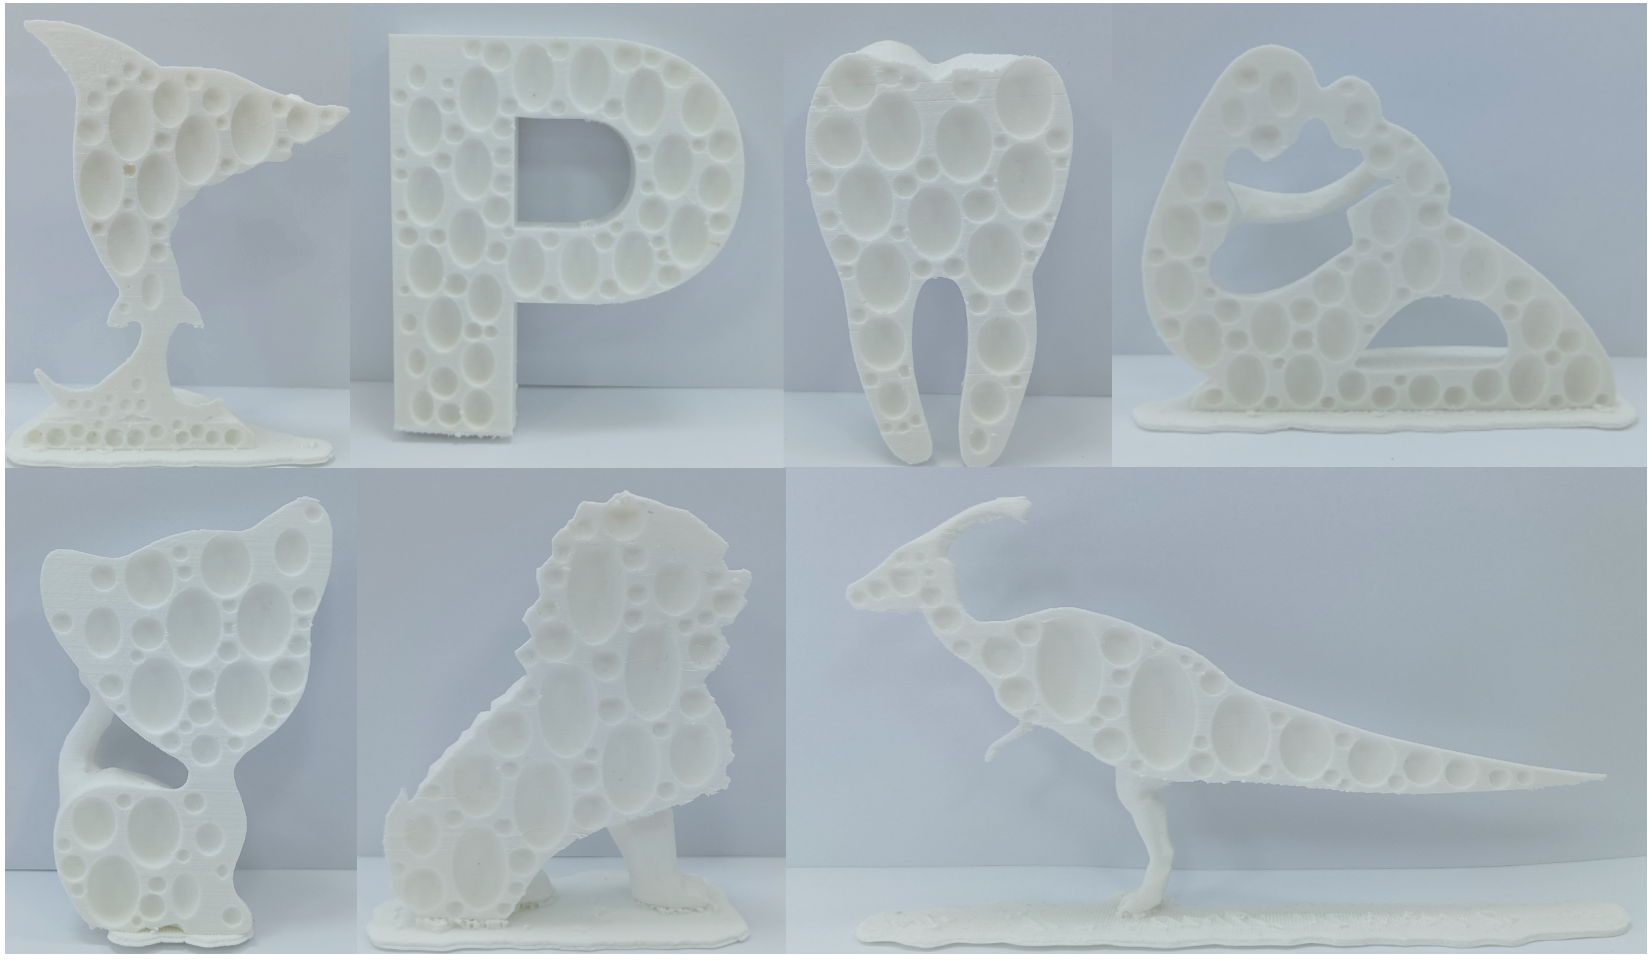
\includegraphics[width=0.9\textwidth]{./figures/self-support/fig16.png}
  \caption{带有椭球形空腔的优化模型的3D打印结果}
  \label{fig:15}
  \end {center}
\end{figure*}

\begin{figure}[htbp]
  \begin {center}
  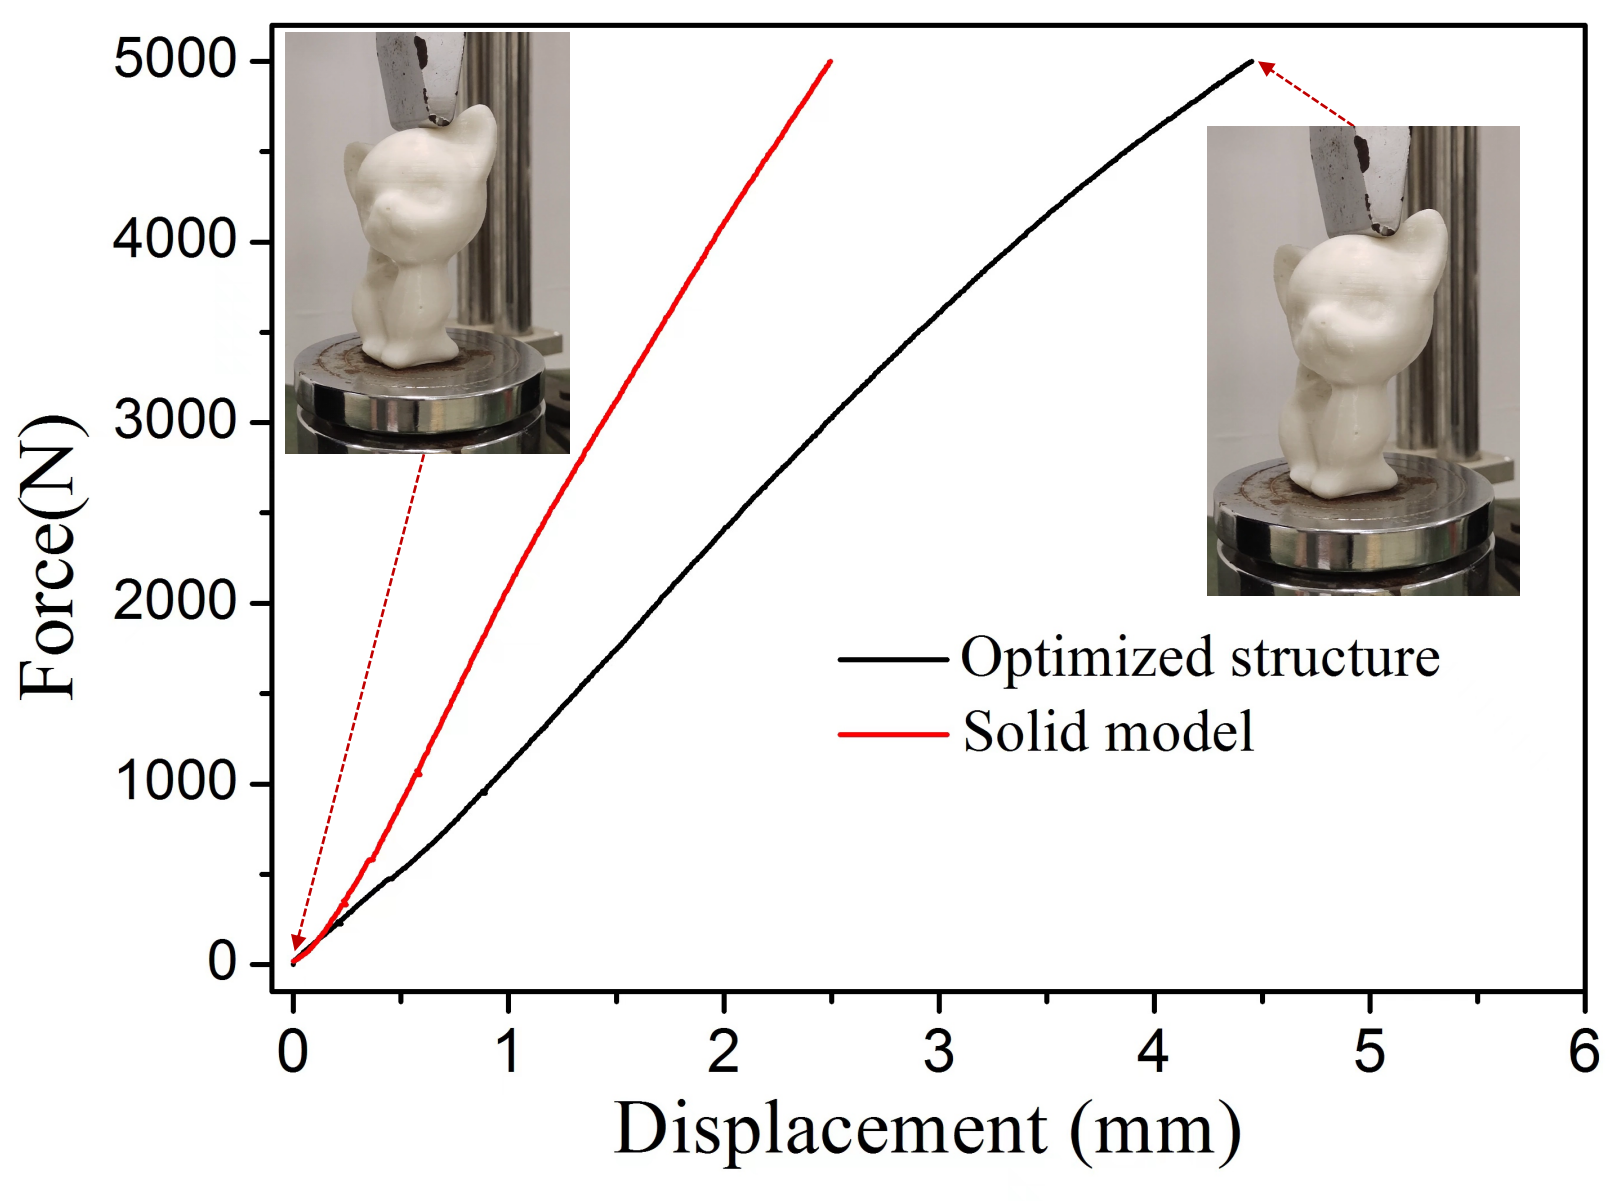
\includegraphics[width=0.6 \textwidth]{./figures/self-support/fig15.png}
  \caption{3D打印模型的实际应力测试 }
  \label{fig:16}
  \end {center}
\end{figure}

\section{本章小结}
本章节提出了一种基于椭球雕刻的无网格自支撑空心化框架。
与现有基于有限元的方法相比,该框架直接在连续函数上进行自支撑空心化的设计和优化,无需耗时的重网格化,大幅提高了空心化问题的有效性和效率。
该框架可自动优化椭球形空腔的形状、位置和拓扑结构,从而得到性能优异的优化自支撑结构。
一系列实验结果证明了该框架的有效性。
% !TeX root = ../thuthesis-example.tex

\chapter{基于隐式神经表示的端到端拓扑优化方法}

% % !TeX root = ../thuthesis-example.tex

\chapter{引用文献的标注}

模板支持 BibTeX 和 BibLaTeX 两种方式处理参考文献。
下文主要介绍 BibTeX 配合 \pkg{natbib} 宏包的主要使用方法。


\section{顺序编码制}

在顺序编码制下,默认的 \cs{cite} 命令同 \cs{citep} 一样,序号置于方括号中,
引文页码会放在括号外。
统一处引用的连续序号会自动用短横线连接。

\thusetup{
  cite-style = super,
}
\noindent
\begin{tabular}{l@{\quad$\Rightarrow$\quad}l}
  \verb|\cite{zhangkun1994}|               & \cite{zhangkun1994}               \\
  \verb|\citet{zhangkun1994}|              & \citet{zhangkun1994}              \\
  \verb|\citep{zhangkun1994}|              & \citep{zhangkun1994}              \\
  \verb|\cite[42]{zhangkun1994}|           & \cite[42]{zhangkun1994}           \\
  \verb|\cite{zhangkun1994,zhukezhen1973}| & \cite{zhangkun1994,zhukezhen1973} \\
\end{tabular}


也可以取消上标格式,将数字序号作为文字的一部分。
建议全文统一使用相同的格式。

\thusetup{
  cite-style = inline,
}
\noindent
\begin{tabular}{l@{\quad$\Rightarrow$\quad}l}
  \verb|\cite{zhangkun1994}|               & \cite{zhangkun1994}               \\
  \verb|\citet{zhangkun1994}|              & \citet{zhangkun1994}              \\
  \verb|\citep{zhangkun1994}|              & \citep{zhangkun1994}              \\
  \verb|\cite[42]{zhangkun1994}|           & \cite[42]{zhangkun1994}           \\
  \verb|\cite{zhangkun1994,zhukezhen1973}| & \cite{zhangkun1994,zhukezhen1973} \\
\end{tabular}



\section{著者-出版年制}

著者-出版年制下的 \cs{cite} 跟 \cs{citet} 一样。

\thusetup{
  cite-style = author-year,
}
\noindent
\begin{tabular}{@{}l@{$\Rightarrow$}l@{}}
  \verb|\cite{zhangkun1994}|                & \cite{zhangkun1994}                \\
  \verb|\citet{zhangkun1994}|               & \citet{zhangkun1994}               \\
  \verb|\citep{zhangkun1994}|               & \citep{zhangkun1994}               \\
  \verb|\cite[42]{zhangkun1994}|            & \cite[42]{zhangkun1994}            \\
  \verb|\citep{zhangkun1994,zhukezhen1973}| & \citep{zhangkun1994,zhukezhen1973} \\
\end{tabular}

\vskip 2ex
\thusetup{
  cite-style = super,
}
注意,引文参考文献的每条都要在正文中标注
\cite{zhangkun1994,zhukezhen1973,dupont1974bone,zhengkaiqing1987,%
  jiangxizhou1980,jianduju1994,merkt1995rotational,mellinger1996laser,%
  bixon1996dynamics,mahui1995,carlson1981two,taylor1983scanning,%
  taylor1981study,shimizu1983laser,atkinson1982experimental,%
  kusch1975perturbations,guangxi1993,huosini1989guwu,wangfuzhi1865songlun,%
  zhaoyaodong1998xinshidai,biaozhunhua2002tushu,chubanzhuanye2004,%
  who1970factors,peebles2001probability,baishunong1998zhiwu,%
  weinstein1974pathogenic,hanjiren1985lun,dizhi1936dizhi,%
  tushuguan1957tushuguanxue,aaas1883science,fugang2000fengsha,%
  xiaoyu2001chubanye,oclc2000about,scitor2000project%
}。



% 其他部分
\backmatter

% 参考文献
% \bibliography{ref/refs}  % 参考文献使用 BibTeX 编译
% \printbibliography       % 参考文献使用 BibLaTeX 编译
% \section{参考文献}
\printbibliography
% 附录
% 本科生需要将附录放到声明之后,个人简历之前
% \appendix
% % !TeX root = ../thuthesis-example.tex

\begin{survey}
\label{cha:survey}

\title{Title of the Survey}
\maketitle


\tableofcontents


本科生的外文资料调研阅读报告。


\section{Figures and Tables}

\subsection{Figures}

An example figure in appendix (Figure~\ref{fig:appendix-survey-figure}).

\begin{figure}
  \centering
  \includegraphics[width=0.6\linewidth]{example-image-a.pdf}
  \caption{Example figure in appendix}
  \label{fig:appendix-survey-figure}
\end{figure}


\subsection{Tables}

An example table in appendix (Table~\ref{tab:appendix-survey-table}).

\begin{table}
  \centering
  \caption{Example table in appendix}
  \begin{tabular}{ll}
    \toprule
    File name       & Description                                         \\
    \midrule
    thuthesis.dtx   & The source file including documentaion and comments \\
    thuthesis.cls   & The template file                                   \\
    thuthesis-*.bst & BibTeX styles                                       \\
    thuthesis-*.bbx & BibLaTeX styles for bibliographies                  \\
    thuthesis-*.cbx & BibLaTeX styles for citations                       \\
    \bottomrule
  \end{tabular}
  \label{tab:appendix-survey-table}
\end{table}


\section{Equations}

An example equation in appendix (Equation~\eqref{eq:appendix-survey-equation}).
\begin{equation}
  \frac{1}{2 \uppi \symup{i}} \int_\gamma f = \sum_{k=1}^m n(\gamma; a_k) \mathscr{R}(f; a_k)
  \label{eq:appendix-survey-equation}
\end{equation}


\section{Citations}

Example citations in appendix.
\cite{abrahams99tex}
\cite{salomon1995advanced}
\cite{abrahams99tex,salomon1995advanced}


\bibliographystyle{unsrtnat}
\bibliography{ref/appendix}

\end{survey}
       % 本科生:外文资料的调研阅读报告
% % !TeX root = ../thuthesis-example.tex

\begin{translation}
\label{cha:translation}

\title{书面翻译题目}
\maketitle

\tableofcontents


本科生的外文资料书面翻译。


\section{图表示例}

\subsection{图}

附录中的图片示例(图~\ref{fig:appendix-translation-figure})。

\begin{figure}
  \centering
  \includegraphics[width=0.6\linewidth]{example-image-a.pdf}
  \caption{附录中的图片示例}
  \label{fig:appendix-translation-figure}
\end{figure}


\subsection{表格}

附录中的表格示例(表~\ref{tab:appendix-translation-table})。

\begin{table}
  \centering
  \caption{附录中的表格示例}
  \begin{tabular}{ll}
    \toprule
    文件名          & 描述                         \\
    \midrule
    thuthesis.dtx   & 模板的源文件,包括文档和注释 \\
    thuthesis.cls   & 模板文件                     \\
    thuthesis-*.bst & BibTeX 参考文献表样式文件    \\
    thuthesis-*.bbx & BibLaTeX 参考文献表样式文件  \\
    thuthesis-*.cbx & BibLaTeX 引用样式文件        \\
    \bottomrule
  \end{tabular}
  \label{tab:appendix-translation-table}
\end{table}


\section{数学公式}

附录中的数学公式示例(公式\eqref{eq:appendix-translation-equation})。
\begin{equation}
  \frac{1}{2 \uppi \symup{i}} \int_\gamma f = \sum_{k=1}^m n(\gamma; a_k) \mathscr{R}(f; a_k)
  \label{eq:appendix-translation-equation}
\end{equation}


\section{文献引用}

文献引用示例\cite{abrahams99tex}。


\appendix

\section{附录}

附录的内容。


% 书面翻译的参考文献
\bibliographystyle{unsrtnat}
\bibliography{ref/appendix}

% 书面翻译对应的原文索引
\begin{translation-index}
  \nocite{salomon1995advanced}
  \bibliographystyle{unsrtnat}
  \bibliography{ref/appendix}
\end{translation-index}

\end{translation}
  % 本科生:外文资料的书面翻译
% % !TeX root = ../thuthesis-example.tex

\chapter{补充内容}

附录是与论文内容密切相关、但编入正文又影响整篇论文编排的条理和逻辑性的资料,例如某些重要的数据表格、计算程序、统计表等,是论文主体的补充内容,可根据需要设置。

附录中的图、表、数学表达式、参考文献等另行编序号,与正文分开,一律用阿拉伯数字编码,
但在数码前冠以附录的序号,例如“图~\ref{fig:appendix-figure}”,
“表~\ref{tab:appendix-table}”,“式\eqref{eq:appendix-equation}”等。


\section{插图}

% 附录中的插图示例(图~\ref{fig:appendix-figure})。

\begin{figure}
  \centering
  \includegraphics[width=0.6\linewidth]{example-image-a.pdf}
  \caption{附录中的图片示例}
  \label{fig:appendix-figure}
\end{figure}


\section{表格}

% 附录中的表格示例(表~\ref{tab:appendix-table})。

\begin{table}
  \centering
  \caption{附录中的表格示例}
  \begin{tabular}{ll}
    \toprule
    文件名          & 描述                         \\
    \midrule
    thuthesis.dtx   & 模板的源文件,包括文档和注释 \\
    thuthesis.cls   & 模板文件                     \\
    thuthesis-*.bst & BibTeX 参考文献表样式文件    \\
    thuthesis-*.bbx & BibLaTeX 参考文献表样式文件  \\
    thuthesis-*.cbx & BibLaTeX 引用样式文件        \\
    \bottomrule
  \end{tabular}
  \label{tab:appendix-table}
\end{table}


\section{数学表达式}

% 附录中的数学表达式示例(式\eqref{eq:appendix-equation})。
\begin{equation}
  \frac{1}{2 \uppi \symup{i}} \int_\gamma f = \sum_{k=1}^m n(\gamma; a_k) \mathscr{R}(f; a_k)
  \label{eq:appendix-equation}
\end{equation}


\section{参考文献}

附录中的参考文献示例(\cite{carlson1981two} 和 \cite{carlson1981two,taylor1983scanning,taylor1981study})。

\printbibliography


% 致谢
% !TeX root = ../thuthesis-example.tex

\begin{acknowledgements}
  衷心感谢导师×××教授和物理系××副教授对本人的精心指导。他们的言传身教将使我终生受益。

  在美国麻省理工学院化学系进行九个月的合作研究期间,承蒙 Robert Field 教授热心指导与帮助,不胜感激。

  感谢×××××实验室主任×××教授,以及实验室全体老师和同窗们学的热情帮助和支持!

  本课题承蒙国家自然科学基金资助,特此致谢。
\end{acknowledgements}


% 声明
\statement
% 将签字扫描后的声明文件 scan-statement.pdf 替换原始页面
% \statement[file=scan-statement.pdf]
% 本科生编译生成的声明页默认不加页脚,插入扫描版时再补上;
% 研究生编译生成时有页眉页脚,插入扫描版时不再重复。
% 也可以手动控制是否加页眉页脚
% \statement[page-style=empty]
% \statement[file=scan-statement.pdf, page-style=plain]

% 个人简历、在学期间完成的相关学术成果
% 本科生可以附个人简历,也可以不附个人简历
% !TeX root = ../thuthesis-example.tex

\begin{resume}

  \section*{个人简历}

  197× 年 ×× 月 ×× 日出生于四川××县。

  1992 年 9 月考入××大学化学系××化学专业,1996 年 7 月本科毕业并获得理学学士学位。

  1996 年 9 月免试进入清华大学化学系攻读××化学博士至今。


  \section*{在学期间完成的相关学术成果}

  \subsection*{学术论文}

  \begin{achievements}
    \item Yang Y, Ren T L, Zhang L T, et al. Miniature microphone with silicon-based ferroelectric thin films[J]. Integrated Ferroelectrics, 2003, 52:229-235.
    \item 杨轶, 张宁欣, 任天令, 等. 硅基铁电微声学器件中薄膜残余应力的研究[J]. 中国机械工程, 2005, 16(14):1289-1291.
    \item 杨轶, 张宁欣, 任天令, 等. 集成铁电器件中的关键工艺研究[J]. 仪器仪表学报, 2003, 24(S4):192-193.
    \item Yang Y, Ren T L, Zhu Y P, et al. PMUTs for handwriting recognition. In press[J]. (已被Integrated Ferroelectrics录用)
  \end{achievements}


  \subsection*{专利}

  \begin{achievements}
    \item 任天令, 杨轶, 朱一平, 等. 硅基铁电微声学传感器畴极化区域控制和电极连接的方法: 中国, CN1602118A[P]. 2005-03-30.
    \item Ren T L, Yang Y, Zhu Y P, et al. Piezoelectric micro acoustic sensor based on ferroelectric materials: USA, No.11/215, 102[P]. (美国发明专利申请号.)
  \end{achievements}

\end{resume}


% 指导教师/指导小组评语
% 本科生不需要
% !TeX root = ../thuthesis-example.tex

\begin{comments}
% \begin{comments}[name = {指导小组评语}]
% \begin{comments}[name = {Comments from Thesis Supervisor}]
% \begin{comments}[name = {Comments from Thesis Supervision Committee}]

  论文提出了……

\end{comments}


% 答辩委员会决议书
% 本科生不需要
% !TeX root = ../thuthesis-example.tex

\begin{resolution}

  论文提出了……

  论文取得的主要创新性成果包括:

  1. ……

  2. ……

  3. ……

  论文工作表明作者在×××××具有×××××知识,具有××××能力,论文××××,答辩××××。

  答辩委员会表决,(×票/一致)同意通过论文答辩,并建议授予×××(姓名)×××(门类)学博士/硕士学位。

\end{resolution}


% 本科生的综合论文训练记录表(扫描版)
% \record{file=scan-record.pdf}

\end{document}
